%Paquetes.
\documentclass[10pt,twoside,a4paper]{book}
\usepackage[utf8]{inputenc}
\usepackage[spanish]{babel}
\usepackage{graphicx}
\usepackage{subfigure}
\usepackage[hidelinks]{hyperref}
\usepackage[right=2.5cm]{geometry}
\usepackage{multirow}
\usepackage{float}

% Comienza el documento.
\begin{document}
\pagestyle{empty}

\begin{center}
{\bf\large UNIVERSIDADE DE SANTIAGO DE COMPOSTELA}

\vspace{0.5cm}
{\bf\large ESCOLA TÉCNICA SUPERIOR DE ENXEÑARÍA}

\vspace{1.5cm}

\includegraphics[width=5cm]{figuras/logo_usc.jpg}

\vspace{2cm}
{\bf\Large Plataforma Web para la Validación de Experimentación en Aprendizaje Automático y Minería de Datos}

\vspace{1cm}
{\normalsize TRABAJO DE FIN DE GRADO}
\end{center}

\begin{flushright}
\vspace{6cm}
{\bf Realizado por:} \\
Adrián Canosa Mouzo \\
~ \\
{\bf Dirigido por:} \\
Ismael Rodríguez Fernández \\
Alberto J. Bugarín Díz \\
Manuel Mucientes Molina \\
\end{flushright}


\cleardoublepage
\chapter*{Agradecimientos}

\thispagestyle{empty}

\textit{El presente Trabajo Fin de Grado se ha desarrollado en el marco del proyecto de I+D+i ``QTEMP: Descripción lingüística de fenómenos complejos: cuantificadores borrosos generalizados en proposiciones temporales (TIN2011-29827-C02-02)", coordinado entre el Grupo de Sistemas Intelixentes de la USC y el European Centre for Soft Computing, y financiado por el Ministerio de Economía y Competitividad en el período 2012-2014.}
\cleardoublepage

% Numeración y cabeceras.
\pagenumbering{roman}
\setcounter{page}{1}
\pagestyle{plain}
\tableofcontents
\listoffigures

% Ahora se incluyen los capítulos. Se cambia la numeración y las cabeceras.
\cleardoublepage
\pagenumbering{arabic}
\setcounter{page}{1}
\pagestyle{headings}
%***************************************************************************************************************************

\chapter{Introducción}
En el contexto tecnológico actual, en donde el Big Data es un recurso cada vez más utilizado, el rol
del analista de datos (data scientist) se está convirtiendo en una profesión emergente y de elevada
demanda. Un analista de datos es aquel profesional que reúne, analiza e interpreta los datos obtenidos
con el objetivo de sacar ciertas conclusiones de ellos y así tomar diferentes decisiones, con las que
aumentar la productividad en una organización. Relacionado con el analista de datos, un nuevo rol emergente
en muchas empresas es el de CDO (\textit{``Chief Data Officer"}). Este rol es el responsable de la gestión
y la utilización de la información como un activo para toda la empresa. El analista de datos combina diferentes
habilidades, especialmente las técnicas de la minería de datos y del aprendizaje automático (DM\&ML).

Según Mitchell \cite{mitchell}, una definición de aprendizaje automático sería la siguiente: un programa
de ordenador aprende a partir de una experiencia E a realizar una tarea T (de acuerdo con una medida de
rendimiento P), si su rendimiento al realizar T, medido con P, mejora gracias a la experiencia E. La
minería de datos, por otra parte, es un campo de las ciencias de la computación referido al proceso que trata
de descubrir patrones en grandes volúmenes de conjuntos de datos \cite{mineria}. Para ello utiliza, entre
otros métodos, técnicas estadísticas para deducir estos patrones y tendencias que existen en los datos. Por
lo general, estos patrones no pueden ser detectados mediante exploración tradicional debido a la complejidad o
la gran cantidad de datos.

Una de las tareas más importantes que se deben llevar a cabo en el aprendizaje automático es la
validación de resultados obtenidos por los algoritmos de aprendizaje. El método estándar más aceptado
en la actualidad es el de la aplicación de test estadísticos sobre los experimentos, que, entre otras
utilidades, apoyan la toma de decisiones, como por ejemplo la elección del algoritmo más adecuado.

En este proyecto hemos creado y desarrollado una plataforma para asistir al analista de
datos en el proceso de validación de resultados. Para ello, se extendió una librería de test
estadísticos, se crearon servicios web para facilitar su consulta y se desarrolló una interfaz web
que hace uso de estos servicios. El objetivo es que el analista pueda introducir en la web los datos obtenidos
mediante experimentación y seleccionar el test estadístico que desee utilizar para que, de forma automática, la
plataforma muestre los resultados de la aplicación del test. Así, la plataforma permitirá de un modo fácil y
centralizado la validación de resultados mediante el uso de test estadísticos.

La herramienta se incorporará en la lista de aplicaciones disponibles a través de la web del
CiTIUS para su acceso. El impacto y difusión del resultado del proyecto tiene el potencial de ser amplio,
ya que en la actualidad no existe ninguna herramienta que centralice la aplicación de los test estadísticos de
mayor utilidad para la validación de algoritmos de aprendizaje automático y que, además, resulte fácil de usar.

%***************************************************************************************************************************

\section{Objetivos del proyecto}
El proyecto se centra en crear y desarrollar una plataforma web para asistir al analista de datos
en el proceso de validación de los resultados obtenidos de diferentes algoritmos de aprendizaje. Para ello,
habrá que realizar las siguientes tareas:
\begin{enumerate}
\item Completar y extender una librería de test estadísticos, actualmente implementada en el lenguaje Python.

La librería estará formada por test paramétricos, test para evaluar las condiciones de aplicación de los test
paramétricos (para la normalidad y homocedasticidad), así como test no paramétricos. Estos test se verán en
detalle a lo largo del capítulo \ref{contraste} en las secciones \ref{parametricos}, \ref{condiciones} y
\ref{no_parametricos} respectivamente. La librería a extender se denomina ``nonparametric.py", y los test de
normalidad y homocedasticidad, así como la prueba  $\mathcal{T}$ de Student se tomarán de la librería de estadística
de Python SciPy (scipy.stats). El listado de test para el proyecto es el siguientes:

- Normalidad: Shapiro-Wilk, D’Agostino–Pearson y Kolmogorov–Smirnov.

- Homocedasticidad: Levene.

- Paramétricos: t-test, ANOVA, Bonferroni.

- No paramétricos: Wilcoxon, Friedman, Iman-Davenport, Rangos Alineados de Friedman, Quade, Bonferroni-Dunn,
Holm, Finner, Hochberg, Li, Shaffer.

\item Crear los servicios web en Python, basados en REST, que hagan disponible el acceso a los
test estadísticos vía web.

Los servicios REST están basados en los métodos HTTP (POST y GET para este proyecto). Asimismo, las peticiones
a los servicios web de los test incluirán todos los datos necesarios (petición completa e independiente) para
que el servidor no tenga que mantener ningún estado para procesar la petición. Los datos a transmitir (datos del
analista, resultados obtenidos por los test) con REST se podrán transferir mediante XML, JavaScript Object
Notation (JSON), o ambos. Cada servicio dispondrá de varias URIs distintas en función de los parámetros para dar
mayor versatilidad a la API.

\item Desarrollar una interfaz web (HTML + JavaScript) para facilitar el uso de los test sobre los
datos introducidos por el analista de datos.

Las tecnologías que se emplearán para desarrollarla serán: HTML, JavaScript y CSS. Un requisito para el proyecto
es que el analista pueda aplicar los test de la forma más sencilla posible, por lo que se tendrá en cuenta este
aspecto en el desarrollo.
\end{enumerate}

%***************************************************************************************************************************

\section{Organización del documento}
La finalidad de este documento es la de presentar los desarrollos realizados para resolver correctamente los objetivos definidos, explicando para ello cada una de las partes que componen la plataforma web y las tareas realizadas a lo largo del proceso.
\begin{itemize}
\item En el \textit{\textbf{capítulo 2}} se explican los conceptos básicos manejados en el proyecto. Para ello, se realiza un análisis detallado del contraste de hipótesis, tratando los conceptos básicos con ejemplos. Además, se explica la finalidad y funcionamiento de cada uno de los test disponibles en la plataforma.
\item El \textit{\textbf{capítulo 3}} hace un análisis de los requisitos identificados en el proyecto, utilizando para ello las historias de usuario empleadas en la metodología del proyecto.
\item El \textit{\textbf{capítulo 4}} describe la gestión del proyecto. Incluye el análisis de riesgos, la metodología de desarrollo, la gestión de la configuración, la planificación temporal y el análisis de costes.
\item En el \textit{\textbf{capítulo 5}} se propone una arquitectura a alto nivel del sistema y se definen cada una
de las partes de las que constará, así como las herramientas de diseño y desarrollo utilizadas.
\item El \textit{\textbf{capítulo 6}} explica tanto el diseño como la implementación a bajo nivel de la arquitectura
propuesta.
\item El \textit{\textbf{capítulo 7}} se definen las pruebas establecidas para poder comprobar que la herramienta es válida y que los objetivos se han cumplido. Se detallan además los resultados de las mismas.
\item Por último, en el \textit{\textbf{capítulo 8}} se establecen aquellas conclusiones derivadas de la realización del
proyecto, además de una breve indicación de lo que podría ser mejorable o ampliable en un futuro.
\end{itemize}

%***************************************************************************************************************************
\cleardoublepage
%***************************************************************************************************************************

\chapter{Contraste de hipótesis} \label{contraste}
El contraste de hipótesis, también conocido como test estadísticos, se engloba en el ámbito de la
Inferencia Estadística, que es la parte de la estadística que estudia cómo sacar conclusiones generales
(sujetas a un determinado grado de fiabilidad o significancia) para toda la población a partir del
estudio de una muestra. En nuestro caso, se tratará de sacar conclusiones de los resultados obtenidos por
diferentes algoritmos sobre distintos conjuntos de datos para determinar, por ejemplo, si los algoritmos
tienen un rendimiento significativamente diferente y por lo tanto no se pueden considerar iguales.

El \textbf{contraste de hipótesis} es uno de los problemas más comunes dentro de la inferencia
estadística. En él se contrasta una hipótesis estadística. Por ejemplo:\\\\
\textit{Un ingeniero de software afirma que la media de los resultados obtenidos por un algoritmo
de aprendizaje automático es 10. ¿Se podría desmentir la afirmación del ingeniero?}\\\\
El planteamiento del contraste sería el siguiente  ($\mu$ indica media poblacional):
\begin{center}
$ \mu = 10 $

$ \mu \neq 10 $
\end{center}

Para tomar una decisión (desmentir o no la afirmación), hay que basarse en los datos de una muestra, para
comprobar si en efecto la media de los resultados es 10 (media muestral). Para ello, se podría establecer una
regla de decisión sobre la cual se basaría nuestra decisión final. Por ejemplo: si la media obtenida está
próxima a la indicada por el ingeniero (10), entonces se podría afirmar que dice la verdad. Si por el
contrario la muestra nos proporciona una media muy distinta a 10, entonces se puede concluir que la evidencia
desmiente la afirmación del ingeniero sobre el algoritmo en cuestión. Esto plantea cuándo  se puede considerar
que la media es lo suficientemente distinta como para determinar que la afirmación del ingeniero es errónea. Por
ejemplo si la media de la muestra es 8.5, ¿se podría desmentir la afirmación inicial? El contraste de hipótesis
nos proporciona una forma de establecer este criterio y poder rechazar o aceptar la afirmación inicial.

%***************************************************************************************************************************

\section{Hipótesis nula y alternativa}
En todo contraste de hipótesis siempre se dan dos posibilidades o hipótesis, las cuales se representan con
los siguientes símbolos:
\begin{center}
$H_0:$ hipótesis nula

$H_1:$ hipótesis alternativa
\end{center}
\begin{itemize}
\item $H_0$: es la hipótesis que se supone cierta de partida, es decir, es la hipótesis que establece que lo que
indica la muestra es solamente debido a la variación aleatoria entre la muestra y la población.
\item $H_1$: es la hipótesis alternativa y es la que reemplazará a la hipótesis nula si ésta es rechazada. $H_1$
establece que lo que indica la muestra es verdadero, y representa a toda la población.
\end{itemize}
A modo de ejemplo, supongamos que unos programadores están trabajando en la optimización de un algoritmo
de aprendizaje. El objetivo es mejorar el algoritmo de forma que los resultados que proporcione sean menores
de 100. Se toma una muestra de los resultados obtenidos por el nuevo algoritmo optimizado y se observa que la
media de la muestra es de 92. Si no hubiera incertidumbre en la media muestral, entonces se podría concluir
que la modificación reduciría los resultados a 92. Sin embargo, siempre existe incertidumbre en la media
muestral. La media poblacional en realidad será poco mayor o menor a 92.

Los programadores están preocupados de que el nuevo algoritmo en realidad no mejore al anterior, es decir, que
la media poblacional pudiera ser mayor o igual a 100. Quieren saber si esta preocupación está justificada. Se ha
observado una muestra con media de 92 y existen dos posibles interpretaciones, o como se ha mencionado más arriba,
dos tipos de hipótesis que serán contrastadas más adelante mediante un determinado test estadístico:
\begin{enumerate}
\item La media poblacional es mayor o igual a 100 (la media muestral es, por tanto, menor debido sólo a la
variación aleatoria de la media poblacional). El nuevo algoritmo no mejorará al anterior.
\item La media poblacional es menor que 100, y la media muestral lo refleja. El nuevo algoritmo sí mejorará
al anterior.
\end{enumerate}
La primera interpretación sería la hipótesis nula o $H_0$. La segunda, la hipótesis alternativa o $H_1$, como se
comentó más arriba.

En este caso, los programadores están preocupados de que la hipótesis nula sea cierta. Un test estadístico o
prueba de hipótesis hallará una medida cuantitativa de la factibilidad de la hipótesis nula (denominado
estadístico de contraste, que para este ejemplo viene dado por la media obtenida en la muestra) y se podrá
decir a los programadores (después de que el test tome la decisión) si su preocupación está o no justificada.
Por tanto, a modo de resumen este ejemplo nos proporciona dos hipótesis:
$$H_0: \mu \geq 100 \mbox{ vs. } H_1: \mu < 100$$

La realización de un contraste de hipótesis no consiste en decidir cuál de las dos hipótesis ($H_0$, $H_1$) es más
creíble, sino en decidir si la muestra proporciona o no suficiente evidencia para descartar $H_0$. Para realizar la
prueba de hipótesis o test estadístico se pone la hipótesis nula en juicio, es decir se empieza suponiendo que $H_0$
es verdadera. Se podría poner como analogía el supuesto de \textit{``En un juicio, el acusado siempre es inocente
hasta que se demuestre lo contrario."} Esto es:
\begin{center}
$H_0:$ el acusado es inocente

$H_1:$ el acusado es culpable
\end{center}
y, mientras no se tenga suficiente evidencia para aceptar $H_1$, hay que creer que lo que dice $H_0$ es cierto. La
muestra aleatoria proporcionará la evidencia. Si el juicio (test o prueba de hipótesis) determina que el acusado
es inocente, sólo se puede decir que no se tiene suficiente evidencia para asegurar que el acusado es culpable,
mientras que si aceptamos la hipótesis alternativa, se estará bastante seguro de que el acusado sí es culpable.

%***************************************************************************************************************************

\section{Estadístico de contraste} \label{estadistico}
Los test estadísticos o pruebas de hipótesis, calculan internamente una medida cuantitativa que proporciona la
factibilidad de la hipótesis nula. Esta medición se extrae de la muestra proporcionada. Por ejemplo, si queremos
contrastar la hipótesis de que la media poblacional es 5, un estadístico a calcular puede ser la media de una
muestra. En este caso, la muestra viene determinada por los resultados obtenidos por los algoritmos y cada uno de
los test tiene una forma particular de hallar este estadístico mediante una fórmula que lo caracteriza. Estos
estadísticos siguen una determinada distribución de probabilidad. Por ejemplo, en este proyecto los test
implementados harán uso de estadísticos que siguen distribuciones como:
\begin{itemize}
\item Distribución normal $\mathcal{N}$ (p. ej. test de Wilcoxon).
\item Distribución chi-cuadrado $\chi^2$ (p. ej. test de Friedman).
\item Distribución $\mathcal{F}$ de Fisher-Snedecor (p. ej. test de Iman-Davenport).
\item Distribución $\mathcal{T}$ de Student (p. ej. t-test).
\end{itemize}
La figura \ref{fig:pdf}, nos muestra el aspecto que presentan las distintas distribuciones de probabilidad. Las
distribuciones dependen de ciertos parámetros para determinar su forma ($\mu$, $\sigma^2$...): 
\begin{figure}[h]
\centering
\subfigure[Distribución $\mathcal{N}$ con media $\mu$ y varianza $\sigma^2$.]{
\label{fig:pdfa}
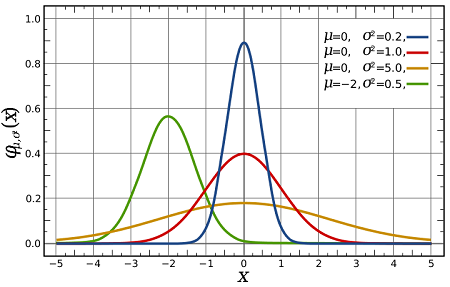
\includegraphics[width=5cm,height=3cm]{figuras/pdf_normal.png} }
\subfigure[Distribución $\chi^2$ con $K$ grados de libertad.]{
\label{fig:pdfb}
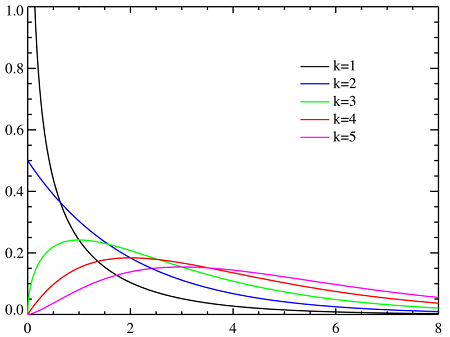
\includegraphics[width=5cm,height=3cm]{figuras/pdf_chi_cuadrado.png} }
\end{figure}
\begin{figure}[h]
\centering
\subfigure[Distribución $\mathcal{F}$ con $d1$ y $d2$ grados de libertad.]{
\label{fig:pdfc}
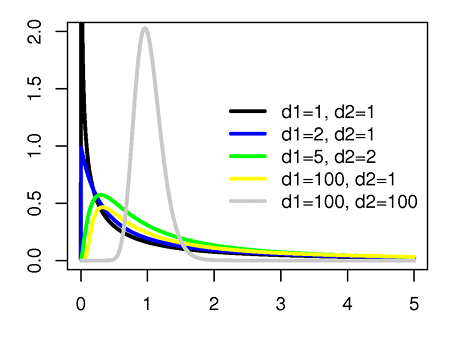
\includegraphics[width=5cm,height=3cm]{figuras/pdf_f.png} }
\subfigure[Distribución $\mathcal{T}$ con $K$ grados de libertad.]{
\label{fig:pdfd}
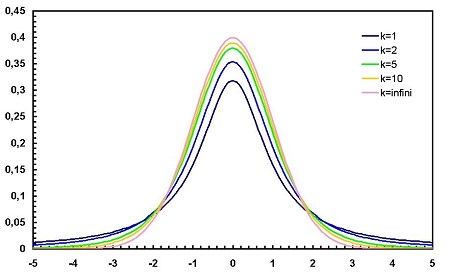
\includegraphics[width=5cm,height=3cm]{figuras/pdf_t_student.jpg} }
\caption{Distribuciones de probabilidad.}
\label{fig:pdf}
\end{figure}
\newline
Como podemos ver en la figura \ref{fig:pdf}, la distribución normal presenta $\mu$ y $\sigma^2$ como parámetros.
Éstos indican media y varianza respectivamente. La varianza, es una medida de dispersión que indica cómo se
distribuye la población. Por ejemplo: en una distribución normal de media 0 y varianza 1 (línea roja en la figura \ref{fig:pdfa}), aproximadamente el $68\%$ de la población se encuentra en el intervalo $[-1,1]$,
ya que el área bajo la curva es de 0.68. Por tanto, la probabilidad de que un individuo de la población se
encuentre en ese intervalo es del 68\%. Si un estadístico sigue una distribución normal con media $\mu$ y
varianza $\sigma^2$, se expresa como:
\[ \mbox{Estadístico} \sim N(\mu,\sigma^2) \]
En las distribuciones $\chi^2$ y $\mathcal{T}$ de Student se habla del parámetro $K$ o grados de libertad ($d1$ y $d2$  en
la distribución $\mathcal{F}$ de Fisher-Snedecor). La media y la varianza de estas tres distribuciones vendrán
determinadas por el parámetro $K$. Cuando se habla de grados de libertad se está haciendo referencia al número de valores
que se pueden elegir libremente en una muestra. Por ejemplo: una muestra con dos datos y media 5 si el primer dato
toma el valor 4 entonces necesariamente el segundo dato debe de ser 6 (para lograr la media de 5). En este caso,
se tienen:
\begin{center}
$N - 1$ grados de libertad, donde $N$ es el tamaño de la muestra.
\end{center}
Se hallan con la fórmula $N-R$, donde $N$ es el número de individuos en la muestra cuyo valor puede ser elegido de
forma libre y $R$ es el número de sujetos cuyo valor dependerá del valor que tengan los individuos de la muestra que
son libres. También se puede representar por $K-R$, donde $K$ es el número de grupos (cuando intervienen grupos y
no sujetos individuales).

En nuestro caso, $N$ viene determinado por el número de resultados obtenidos por los algoritmos (número de filas
de la matriz de la muestra de datos) y $K$ por el número de algoritmos o variables relacionadas que tiene la muestra
de datos con la que se están aplicando los test (número de columnas de la matriz). Cada test que use el parámetro
de grados de libertad lo calcula de acuerdo a su fórmula característica para el estadístico. 

Todas las distribuciones de la figura \ref{fig:pdf} son continuas, pues se puede tomar cualquier valor dentro de un
intervalo, a diferencia de las distribuciones discretas. Por otra parte, en la distribución $\mathcal{T}$ de Student
a medida que aumentan los grados de libertad se tiende más a una distribución normal
estandarizada (de $\mu = 0$ y $\sigma^2 = 1$).

Las distribuciones de probabilidad que pueda seguir un estadístico nos dan un valor diferente de probabilidad para
cada valor diferente del estadístico. Este valor de probabilidad indica cuán probable es obtener ese valor del
estadístico siendo la hipótesis nula cierta. Por ejemplo, si es cierta la hipótesis nula de que la media de una población
es 5, es más probable que obtengamos una media de una muestra igual a 4.5 que a 3.

%***************************************************************************************************************************

\section{Decisiones y tipos de error} \label{tipos_error}
Cuando se lleva a cabo un contraste de hipótesis sólo se pueden tomar dos decisiones. Los datos de la muestra,
que en este proyecto vendrá dada por los resultados obtenidos por los algoritmos, evidenciarán qué decisión se
debe tomar:
\begin{enumerate}
\item Aceptar la hipótesis nula ($H_0$) (rechazar la hipótesis alternativa $H_1$)
\item Rechazar $H_0$ (aceptar la hipótesis alternativa)
\end{enumerate}
Sin embargo, cuando se toma la decisión se pueden cometer dos tipos de errores (fig. \ref{fig:decision}):
\begin{figure}[H]
\centering
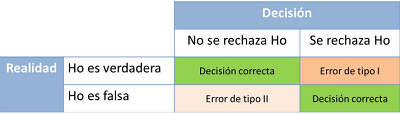
\includegraphics[width=7cm,height=2cm]{figuras/tipos_error.png}
\caption{Decisiones y tipos de error.}
\label{fig:decision}
\end{figure}
La probabilidad de ``Error tipo I" se denota por $\alpha$ y se denomina nivel de significación:
\begin{center}
$P(\mbox{``Error tipo I}") = P(\mbox{Rechazar } H_0|H_0 \mbox{ es cierta}) =\alpha$
\end{center}
El nivel de significación consiste en la probabilidad de rechazar la hipótesis nula $H_0$ cuando verdaderamente
es cierta. Este valor $\alpha$ es un parámetro que debe seleccionar la persona que quiere realizar un test
estadístico en base a cuán importante es rechazar $H_0$ cuando es cierta. Normalmente es del 5\%, lo
que implicará que 5 de cada 100 veces se acepta la hipótesis alternativa cuando la cierta es la hipótesis nula.
Cuanto menor sea el nivel de significación, cada vez es más difícil rechazar la hipótesis nula. Es decir, si
queremos equivocarnos menos veces, necesitamos mucha más evidencia para justificar el rechazo. Si es grande es
más fácil aceptar la hipótesis alternativa cuando en realidad es falsa.
\\Por otra parte, la probabilidad de ``Error tipo II" se denota por $\beta$:
\begin{center}
$P(\mbox{``Error tipo II}") = P(\mbox{Aceptar } H_0|H_0 \mbox{ es falsa}) =\beta$
\end{center}
Este error $\beta$ consiste en la probabilidad de aceptar la hipótesis nula $H_0$ cuando verdaderamente es
falsa.
\\Por último, cabe destacar el concepto de ``Potencia".
\begin{center}
$P(\mbox{``Potencia}") = P(\mbox{Rechazar } H_0|H_0 \mbox{ es falsa}) =1-\beta.$
\end{center}
La potencia es la probabilidad de detectar que una hipótesis es falsa. Los test estadísticos o pruebas de hipótesis
implementados en el presente proyecto se caracterizan por su potencia, siendo esta fija, y dejando como parámetro
libre el nivel de significación. Así, cuanto mayor es el nivel de potencia, mejor será el test, ya que se rechazarán
más hipótesis nulas cuando se deben rechazar (mayor habilidad en aceptar correctamente hipótesis alternativas).

En este proyecto se pondrá el énfasis en el nivel de significación, ya que es la hipótesis alternativa la que se
quiere probar y no se quiere aceptar si en realidad no es cierta es decir, si aceptamos la hipótesis alternativa
queremos equivocarnos con un margen de error muy pequeño. Obviamente, lo ideal sería que tanto $\alpha$ como
$\beta$ fuesen nulos y que no se cometiese ningún error, o que ambos valores fuesen muy pequeños. Como no se pueden
disminuir ambos errores a la vez, se controla el ``Error tipo I".

%***************************************************************************************************************************

\section{Intervalos de confianza}
El nivel de significación fijado divide en dos regiones el conjunto de posibles valores del estadístico de
contraste: la región de aceptación y la región de rechazo o región crítica. Se denomina región de aceptación
a la región que conduce a la aceptación de $H_0$ y región de rechazo a la región que conduce al rechazo de $H_0$
en favor de $H_1$. Aquí surge el concepto de \textbf{Cola}, que indica la porción o porciones de una distribución
de probabilidad en la cual se rechaza la hipótesis nula, es decir, la \textbf{región de rechazo}.

La determinación de las regiones de aceptación o de rechazo depende de cómo se establezca la hipótesis
alternativa $H_1$. Por ejemplo, si hablamos de un contraste en el que se esté contrastando una determinada
media ($\mu_0$) se podría establecer como $H_1$ que la media en realidad sea menor, mayor o distinta a
($\mu_0$):\\\\
\begin{itemize}
\item Media menor (test unilateral con cola a la izquierda):
\end{itemize}
\begin{center}
$H_0: \mu = \mu_0$
\\$H_1: \mu < \mu_0$
\end{center}
\begin{itemize}
\item Media mayor (test unilateral con cola a la derecha):
\end{itemize}
\begin{center}
$H_0: \mu = \mu_0$
\\$H_1: \mu > \mu_0$
\end{center}
\begin{itemize}
\item Media distinta (test bilateral o de dos colas):
\end{itemize}
\begin{center}
$H_0: \mu = \mu_0$
\\$H_1: \mu \neq \mu_0$
\end{center}
En la figura \ref{fig:intervalos_normal}, podemos ver cómo quedarían establecidos los intervalos para el ejemplo. En
rojo se muestra la región de rechazo:
\begin{figure}[h]
\centering
\subfigure[Test unilateral. Cola a la izquierda.]{
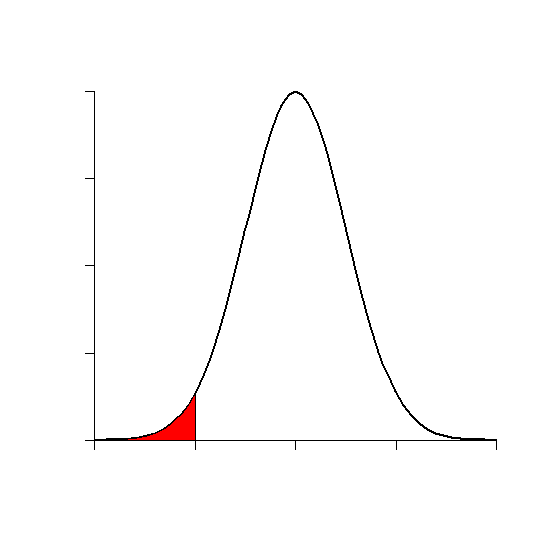
\includegraphics[width=5cm,height=3cm]{figuras/test_unilateral_izq.png} }
\subfigure[Test unilateral. Cola a la derecha.]{
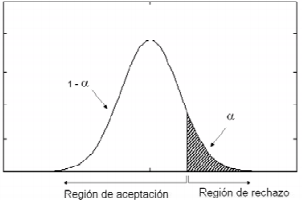
\includegraphics[width=5cm,height=3cm]{figuras/test_unilateral_der.png} }
\end{figure}
\begin{figure}[h]
\centering
\subfigure[Test bilateral o de dos colas.]{
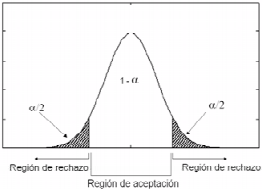
\includegraphics[width=5cm,height=3cm]{figuras/test_bilateral.png} }
\caption{Regiones de aceptación y rechazo.}
\label{fig:intervalos_normal}
\end{figure}

Como se puede observar en el caso del test bilateral o de dos colas, el $\alpha$ se divide en dos porciones iguales:
$\alpha / 2$, que constituyen la región de rechazo. La región de aceptación tendrá en todos los casos probabilidad
$1 - \alpha$.

%***************************************************************************************************************************

\section{Decisión final y \textit{\textit{p-valor}}} \label{pvalor}
Si el valor del estadístico cae en la región de aceptación, se acepta la hipótesis nula, ya que no existen
razones suficientes para rechazar $H_0$ con el nivel de significación dado. Por tanto, en este caso se diría
que el contraste es estadísticamente no significativo, es decir, no existe evidencia estadísticamente significativa
en favor de $H_1$.
\begin{figure}[h]
\centering
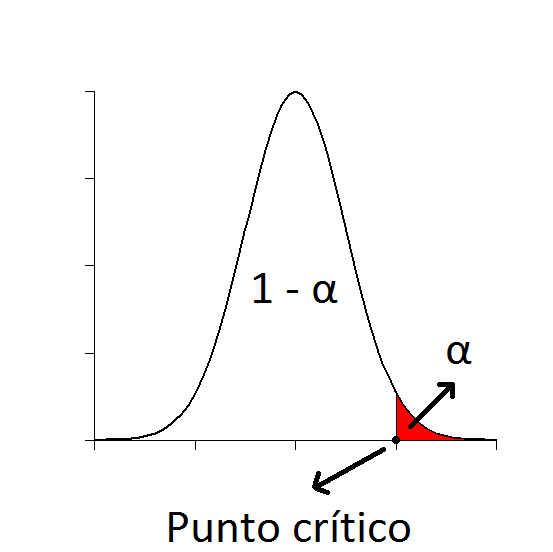
\includegraphics[width=5cm,height=3cm]{figuras/critico.png}
\caption{Punto crítico.}
\label{fig:punto_critico}
\end{figure}
La figura \ref{fig:punto_critico} nos muestra el punto crítico: si el estadístico obtenido por el test o
prueba de hipótesis es 5 y el punto crítico es 4.5, se rechaza $H_0$ ya que el estadístico pertenece a la
región de rechazo.

La decisión de rechazar o aceptar la hipótesis nula, se puede determinar también mediante el $\textit{p-valor}$,
que es el parámetro utilizado para realizar los test estadísticos en este proyecto. El $\textit{p-valor}$ proporciona
un forma más eficiente de determinar si el contraste es o no estadísticamente significativo, ya que no sería
necesario recalcular regiones de aceptación y rechazo cada vez que el usuario de los test cambia de nivel de
significación.

\begin{center}
``El $\textit{p-valor}$, es la probabilidad que hay de obtener un valor al menos tan extremo como el estadístico en cuestión
que se ha calculado."
\end{center}

Para entender mejor el concepto de $\textit{p-valor}$, conviene hablar de las distribuciones de probabilidad vistas en la
figura \ref{fig:pdf} de la sección \ref{estadistico} donde se hablaba del estadístico de contraste. Estas
distribuciones son funciones que se denominan ``funciones de densidad de probabilidad" (FDP). Como expusimos en
la sección \ref{estadistico}, estas funciones proporcionan la probabilidad que existe para cada valor
diferente del estadístico (cuán probable es obtener ese valor del estadístico). Si, en vez de trabajar con las
funciones de densidad de probabilidad, se trabaja con las funciones de distribución acumuladas (FDA), para cada
valor del estadístico éstas devolverían la probabilidad de obtener un valor igual o menor que ese estadístico siendo
la hipótesis nula cierta. En la figura \ref{fig:comparativa_pdf_cdf} podemos ver una comparación entre los dos
tipos de funciones para el caso de la distribución $\chi^2$:

\begin{figure}[h]
\centering
\subfigure[Función de densidad de probabilidad.]{
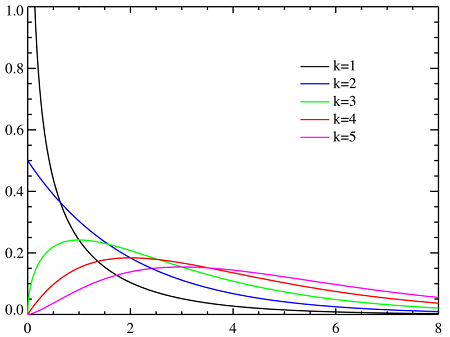
\includegraphics[width=5cm,height=3cm]{figuras/pdf_chi_cuadrado.png} }
\subfigure[Función de distribución acumulada.]{
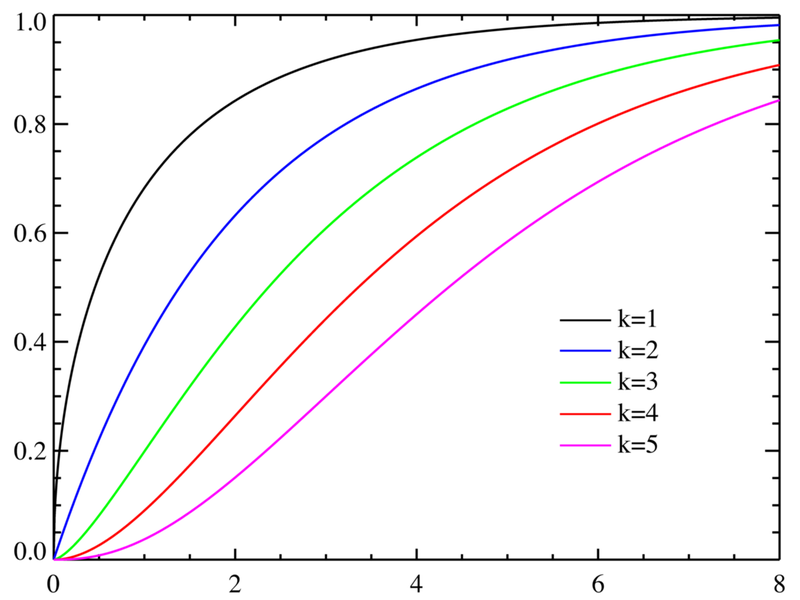
\includegraphics[width=5cm,height=3cm]{figuras/cdf_chi_cuadrado.png} }
\caption{Comparativa entre FDP y FDA.}
\label{fig:comparativa_pdf_cdf}
\end{figure}

Visto de otro modo, con la distribución acumulada, dado un estadístico, nos devuelve la probabilidad que hay de
obtener un valor al menos tan extremo como el estadístico en cuestión. Esto es el \textbf{$\textit{p-valor}$}. Por ejemplo si
el valor del estadístico es 3 y el test da como resultado un $\textit{p-valor}$ igual a 0.1, esto quiere decir que un 10\% de
las veces vamos a obtener un valor similar. Si el $\textit{p-valor}$ es muy bajo, es decir, la probabilidad de obtener un valor
al menos tan extremo como ese estadístico es muy baja, se puede concluir que la hipótesis nula no es cierta, ya que
sería poco probable que siendo cierta se obtuviese ese estadístico.

El criterio para saber si el $\textit{p-valor}$ es lo suficientemente bajo como para rechazar que la hipótesis nula sea cierta
es tomado de acuerdo al nivel de significancia establecido. Como se ha mencionado en la sección \ref{tipos_error}, el
nivel de significancia o $\alpha$ indica la probabilidad de rechazar la hipótesis nula siendo ésta cierta. Si el
$\textit{p-valor}$ es menor que el nivel de significancia se rechaza la hipótesis nula.

Según se disminuye $\alpha$, cada vez es más difícil de rechazar la hipótesis nula, ya que se necesita mucha más
evidencia para justificar el rechazo. Por ejemplo, si $\alpha$ es 0.05 y la probabilidad de obtener un estadístico
igual a 1 es 0.03, se rechaza la hipótesis nula. Sin embargo, si el $\alpha$ fuese 0.01, no se podría rechazar: no hay suficiente evidencia de que la hipótesis nula sea falsa.

%***************************************************************************************************************************

\section{Etapas en la resolución de un contraste de hipótesis}
En un contraste de hipótesis siempre se siguen una serie de pasos definidos. Como se ha ido viendo a lo largo
del capítulo, los pasos para la realización de una prueba de hipótesis o test estadístico son los siguientes
\cite{libro}:
\begin{enumerate}
\item Especificación de la hipótesis nula $H_0$ y de la hipótesis alternativa $H_1$.
\item Suponer que $H_0$ es verdadera (el test sirve para que a partir de la muestra de datos podamos rechazar
$H_0$ en beneficio de $H_1$).
\item Calcular un estadístico de prueba o estadístico de contraste. Este estadístico se usa para evaluar la
fuerza de la evidencia en contra de $H_0$ (medir la discrepancia entre la hipótesis y la muestra).
\item Establecer un nivel de significación $\alpha$ en base a cómo de importante se considere rechazar $H_0$
cuando realmente es verdadera.
\item El nivel de significación fijado divide en dos regiones el conjunto de posibles valores del estadístico
de contraste: la región de aceptación y la región de rechazo o región crítica.
\item Si el valor del estadístico cae en la región de rechazo, se rechaza la hipótesis nula, ya que esto
evidencia que los datos obtenidos de la muestra no son compatibles con $H_0$. Por tanto, en este caso se diría
que el contraste es estadísticamente significativo, es decir, existe evidencia estadísticamente significativa en
favor de $H_1$.
\item Si el valor del estadístico cae en la región de aceptación, se acepta la hipótesis nula, ya que no existen
razones suficientes para rechazar $H_0$ con el nivel de significación dado. Por tanto, en este caso se diría
que el contraste es estadísticamente no significativo, es decir, no existe evidencia estadísticamente significativa
en favor de $H_1$.
\item La decisión de rechazar o aceptar la hipótesis nula, se puede determinar también mediante el $\textit{p-valor}$,
que es el parámetro utilizado para realizar los test estadísticos en este proyecto. El $\textit{p-valor}$ proporciona
un forma más eficiente de determinar si el contraste es o no estadísticamente significativo, ya que no sería
necesario recalcular regiones de aceptación y rechazo cada vez que el usuario de los test cambia de nivel de
significación.
\end{enumerate}

%***************************************************************************************************************************

\section{Tests paramétricos} \label{parametricos}
Uno de los tipos más comunes de test son los test paramétricos. En general, estos test son más robustos y
tienen mayor potencia que los test no paramétricos, que se verán más adelante en la sección \ref{no_parametricos}.
Sin embargo, las pruebas paramétricas se basan en supuestos que muy probablemente se violan cuando se analiza el
rendimiento de algoritmos de optimización y minería de datos \cite{parametricos}. Estas suposiciones
o condiciones paramétricas que deben cumplir los resultados de los algoritmos son explicadas a continuación.

%----------------------------------

\subsection{Condiciones Paramétricas} \label{condiciones}

\subsubsection{Independencia}
En estadística, dos eventos son independientes si cuando uno de ellos se da no modifica la probabilidad de la
ocurrencia del otro. Dicho de otra forma: cuando las muestras o datos obtenidos por los algoritmos, es decir los
resultados de éstos, no dependen unos de otros. La independencia es una característica que en este proyecto debe
asumir el usuario de los test, y, por tanto, podrá actuar de una forma u otra bajo su responsabilidad.

\subsubsection{Normalidad}
Una muestra u observación es normal cuando su comportamiento sigue una distribución normal (o distribución de
Gauss) con una cierta media $\mu$ y varianza $\sigma^2$. En la figura \ref{fig:normalidad} podemos ver que a la
izquierda se cumple el supuesto de normalidad, mientras que a la derecha los datos de la muestra no están distribuidos
de forma normal:

\begin{figure}[h]
\centering
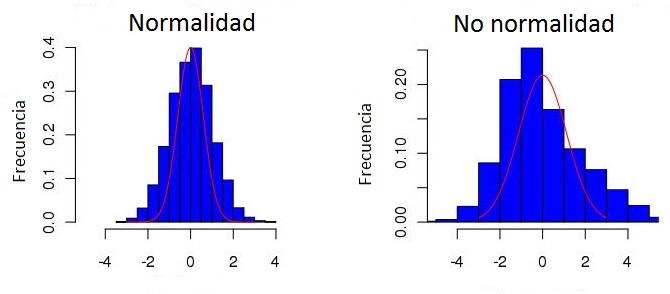
\includegraphics[width=9cm,height=3cm]{figuras/normalidad.jpg}
\caption{Normalidad vs. No normalidad.}
\label{fig:normalidad}
\end{figure}

En este proyecto se pueden realizar los siguientes test no paramétricos para comprobar el supuesto de normalidad:

\begin{itemize}
\item \textbf{Shapiro–Wilk:} contrasta la hipótesis nula de que las muestras o poblaciones provienen de una
población normalmente distribuida. Analiza la muestra para hallar el nivel de simetría y Kurtosis (forma de
la curva) para calcular la diferencia con respecto a una distribución normal, obteniendo el \textit{p-valor} de la suma
de los cuadrados de estas discrepancias. Se considera de los más potentes, sobre todo para muestras de menos
de 30 elementos. Sin embargo, el rendimiento de esta prueba se ve afectado de forma negativa cuando no existe
independencia en los datos.
\item \textbf{D’Agostino–Pearson:} contrasta la hipótesis nula de que las muestras o poblaciones provienen de
una población normalmente distribuida. Primero calcula el coeficiente de asimetría (en qué medida la normal es
simétrica ó coeficiente 0) y el coeficiente de Kurtosis (grado de amplitud, donde lo normal es coeficiente 0) para
cuantificar cuán lejos se está de la distribución normal. Luego, calcula cuánto difiere cada uno de los valores
de los esperados en una distribución normal, para obtener el $\textit{p-valor}$ de la suma de estas discrepancias.
Es menos potente que el test de Shapiro-Wilk, pero no se ve afectado cuando los datos no son independientes.
\item \textbf{Kolmogorov–Smirnov:} realiza una prueba de bondad de ajuste, para determinar si los datos observados
de la muestra se ajustan a la distribución normal. Tiene como $H_0$ que la distribución obtenida de los datos
observados es idéntica a la distribución normal. Es la prueba que menos potencia presenta de los tres, y por tanto
es la que peor funciona.
\end{itemize}

\subsubsection{Homocedasticidad}
La homocedasticidad es la condición que dice que las poblaciones de entrada o datos obtenidos por los algoritmos
proceden de poblaciones con varianzas iguales. Es decir, esta propiedad indica la hipótesis de igualdad de
varianzas. El caso contrario sería heterocedasticidad. En la figura \ref{fig:homocedasticidad} se puede apreciar
la diferencia existente entre unos datos que presentan homocedasticidad y otros que no, donde el eje de ordenadas
representa la varianza del error (la varianza dentro de cada tratamiento o la varianza de los resultados obtenidos
por un algoritmo en los distintos conjuntos de datos), y el eje de abscisas representa a las observaciones. En el
primer caso, la varianza del error se mantiene constante a lo largo de las observaciones, mientras que en el otro
caso no:

\begin{figure}[h]
\centering
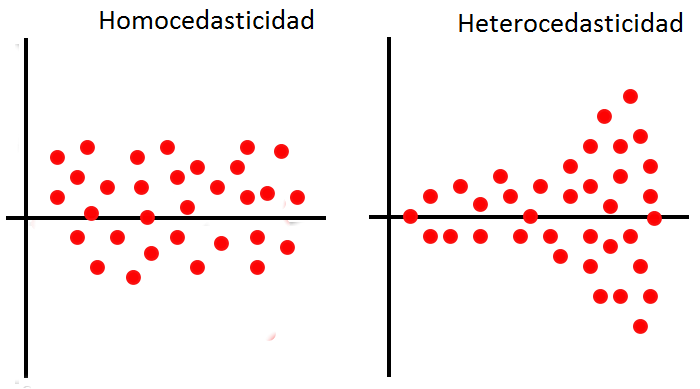
\includegraphics[width=6cm,height=3cm]{figuras/homocedasticidad.png}
\caption{Homocedasticidad vs. Heterocedasticidad.}
\label{fig:homocedasticidad}
\end{figure}

En este proyecto se puede realizar el siguiente test no paramétrico para comprobar el supuesto de homocedasticidad:

\begin{itemize}
\item \textbf{Test de Levene:} contrasta la hipótesis nula de que todas las poblaciones de entrada proceden de
poblaciones con varianzas iguales. Se utiliza para comprobar si K muestras pertenecientes a datos obtenidos por
K algoritmos presentan o no homogeneidad de varianzas. 
\end{itemize}

%----------------------------------

\subsection{Test ANOVA}
El análisis de la varianza (ANOVA) es uno de los test estadísticos más ampliamente utilizados para probar
la igualdad de más de dos medias de la población. Se trata de una versión más general del t-test, ya que permite
comparar más de 2 poblaciones (en este proyecto resultados de más de dos algoritmos). Dado que es un test
paramétrico, se asume que se dan las condiciones de independencia, normalidad y homocedasticidad en su
aplicación. De no ser el caso, los resultados de esta prueba no son fiables.

\subsubsection{Hipótesis}
\begin{itemize}
\item Hipótesis nula $H_0$: $\mu_1 = \mu_2 = \mu_3 ... = \mu_K$.
\item Hipótesis alternativa $H_1$: $\exists \quad \mu_j \neq \mu \quad j=1,2,...,K$.
\end{itemize}
La hipótesis nula indica que las medias de distintas poblaciones o muestras coinciden $(K>2)$, frente a la
hipótesis alternativa de que por lo menos una de las poblaciones tiene una media que difiere de las demás. Es,
por tanto, un contraste o prueba unilateral con cola a la derecha. En este proyecto el parámetro $K$ viene
determinado por el número de algoritmos que existen en la muestra de datos.

\subsubsection{Pasos a desarrollar}
Los pasos a seguir para realizar el test de ANOVA son los siguientes:
\begin{itemize}
\item Se analiza la variación total (respecto a la media general o media de medias de los resultados de cada
algoritmo):
\[ variacion_t = \sum_{i=1}^{N} \sum_{j=1}^{K} (X_{ij} - \bar{X})^2, \]
donde $\bar{X}$ es la media general, $N$ es el número de conjuntos de datos o problemas sobre los que se
aplican los algoritmos y $X_{ij}$ es un resultado específico obtenido por un algoritmo.
\item Se halla también la variación entre los diferentes tratamientos o algoritmos (efecto de la media de cada
tratamiento respecto a la media general):
\[ variacion_{tr} = \sum_{i=1}^{K} N (\bar{X}_i - \bar{X})^2, \]
donde $\bar{X}_i$ representa la media del tratamiento o algoritmo.
\item La variación dentro del tratamiento o variación del error (cada valor respecto a la media de su tratamiento):
\[ variacion_e = \sum_{i=1}^{N} \sum_{j=1}^{K} (X_{ij} - \bar{X}_{j})^2, \]
donde $\bar{X}_{j}$ representa la media de un tratamiento o algoritmo.
\item Se calculan los grados de libertad totales, del tratamiento y del error como:
\[ GLT = (NK)-1 \]
\[ GLTR = K-1 \]
\[ GLE = GLT - GLTR \]
\item Luego se determinan los cuadrados medios totales ($CMT$) del tratamiento ($CMTR$) y del error ($CME$),
que son las variaciones divididas entre los grados de libertad correspondientes.
\item Se halla el estadístico, que se distribuye como una distribución $\mathcal{F}$ con $K-1$ y $(KN)-K$ grados de libertad:
\[ anova = CMT / CME \]
\item Por último se halla el $\textit{p-valor}$ y se toma la decisión en función del nivel de significancia. A modo
de ejemplo para el cálculo del $\textit{p-valor}$ en este caso, primero se haya la probabilidad de obtener un
estadístico menor o igual que el calculado previamente (es decir, el valor que proporciona la función de distribución acumulada $\mathcal{F}$ de Fisher-Snedecor para el estadístico con $K-1$ y $(KN)-K$ grados de libertad, como vimos en
la sección \ref{pvalor}). Esto representaría un área (probabilidad acumulada) en la función de densidad de
probabilidad: el área a la izquierda del valor del estadístico. Dado que se trata de un contraste unilateral con cola
a la derecha, se resta esta probabilidad a la probabilidad total, es decir, a 1, para obtener así el área que queda a la derecha del estadístico. Si este valor resultante ($\textit{p-valor}$) es menor que el nivel de significancia, se
rechazaría la hipótesis nula.

En un contraste bilateral, para hallar el $\textit{p-valor}$ habría que multiplicar el valor devuelto en la función de distribución acumulada por 2, ya que en este caso habría dos colas.
\end{itemize}

%----------------------------------

\subsection{t-test}
El caso más simple de ANOVA donde intervienen únicamente 2 muestras o algoritmos es realizado por este test, también
conocido como la prueba $\mathcal{T}$ de Student. Dado que es un test paramétrico, se asume que se dan las condiciones
de independencia, normalidad y homocedasticidad en su aplicación. De no ser el caso, los resultados de esta prueba no
son fiables.

\subsubsection{Hipótesis}
\begin{itemize}
\item Hipótesis nula $H_0$: $\mu_1 = \mu_2$.
\item Hipótesis alternativa $H_1$: $\mu_1 \neq \mu_2$.
\end{itemize}
La hipótesis nula indica que las medias de las 2 poblaciones o muestras coinciden, frente a la hipótesis alternativa
de que son distintas. Se trata, por tanto, de un contraste o prueba bilateral. El estadístico de este test, sigue una distribución $\mathcal{T}$ de Student con $2N-2$ grados de libertad.

%----------------------------------

%***************************************************************************************************************************

\section{Tests no paramétricos} \label{no_parametricos}
Cuando los datos obtenidos de la aplicación de los algoritmos de aprendizaje automático no cumplen las
características de independencia, normalidad u homocedasticidad total o parcialmente,  es necesario aplicar
test no paramétricos. La validación de nuevos algoritmos requiere con frecuencia la definición de un marco
experimental exhaustivo y la parte crítica de estas comparaciones recae en la validación estadística de los
resultados, contrastando las diferencias encontradas entre métodos. Dentro de las técnicas disponibles, destacan
los test no paramétricos debido a su flexibilidad y a las pocas restricciones de uso que presentan (a diferencia
de los test paramétricos, los cuales sufren a menudo problemas derivados de la imposibilidad de cumplir las
condiciones paramétricas para su uso) \cite{no_parametricos}.

%----------------------------------

\subsection{Test de Wilcoxon}
La prueba de los rangos con signo de Wilcoxon también conocida como el test de Wilcoxon es una prueba no
paramétrica que se utiliza como alternativa a la prueba $\mathcal{T}$ de Student cuando no se puede suponer la normalidad
de las muestras. Es, por tanto, menos potente que que la prueba $\mathcal{T}$ de Student. El test de Wilcoxon fue creado
por Frank Wilcoxon y publicado en 1945 \cite{wilcoxon}.

Sirve para comparar dos métodos o tratamientos (en este proyecto interesa comparar dos algoritmos). Por tanto,
los individuos (los problemas) donde se aplican los algoritmos tienen que ser los mismos. Es decir, a un mismo
individuo se le efectúa la medición de dos variables: las muestras son apareadas. Para tomar la decisión hay
que basarse en las observaciones de N individuos independientes (sin relación existente entre ellos). Para tamaños
muestrales pequeños, se puede determinar mediante la comparación del estadístico con el valor crítico de la
tabla de Wilcoxon. Para tamaños muestrales grandes ($> 25$), el test se puede aproximar con la distribución normal.

\subsubsection{Hipótesis}
\begin{itemize}
\item Hipótesis nula $H_0$: la mediana de las diferencias $ = 0$.
\item Hipótesis alternativa $H_1$: la mediana de las diferencias $ \neq 0$.
\end{itemize}
La mediana, es el valor que ocupa el lugar central de todos los datos cuando éstos están ordenados de menor a
mayor. $H_0$ indica que la mediana de las diferencias de dos muestras (resultados de dos algoritmos) relacionadas
son iguales, es decir, las dos medianas son iguales (los resultados obtenidos no dependen del algoritmo).
$H_1$ indica, por otra parte, que las medianas son diferentes. Se trata, por tanto, de una prueba bilateral.

\subsubsection{Pasos a desarrollar}
Los pasos a seguir para realizar la prueba de los rangos de Wilcoxon son los siguientes:
\begin{itemize}
\item Se calculan las diferencias entre las muestras. Por ejemplo: diferencias entre los resultados del algoritmo
A y B.
\subitem - Se eliminan los elementos que tengan diferencias nulas.
\item Se ordenan las diferencias en valor absoluto (independientemente del signo).
\item Se asignan rangos de orden 1,2,...,N. Si hay empates se calcula la media del rango de cada uno de los elementos
repetidos.
\item Suma de los rangos según los signos que tengan las diferencias para obtener los estimadores:
\subitem - $T(+) = $ Suma de los rangos correspondientes a diferencias positivas. 
\subitem - $T(-) = $ Suma de los rangos correspondientes a diferencias negativas.
\item Definir el estadístico:
\subitem - $T = \min [T(+), T(-)]$
\item Si $N \leq 25$, se examina la tabla de Wilcoxon que nos da los valores críticos (el intervalo de aceptación)
para cada valor de N y cada nivel de significancia. El contraste será estadísticamente significativo si: 
$T <= $ límite inferior correspondiente.
\item Si $N > 25$, el estadístico se ajusta a la distribución normal. Por tanto, se calcula el estadístico $Z$ y
se toma la decisión en función del $\textit{p-valor}$ y del nivel de significancia:
\[ Z = \frac{T-\frac{N(N+1)}{4}}{\sqrt{\frac{N(N+1)(2N+1)}{24}}} \]
\end{itemize}

%----------------------------------

\subsection{Test de Friedman}
El test de Friedman es una prueba no paramétrica que puede realizar comparaciones entre dos o más algoritmos, es
decir, se trata de una prueba de comparaciones múltiples. Fue desarrollada por el economista Milton Friedman y
trabaja asignando rankings para establecer cuál es el mejor algoritmo de la muestra de datos proporcionada.

\subsubsection{Hipótesis}
\begin{itemize}
\item Hipótesis nula $H_0$: no existen diferencias entre los algoritmos.
\item Hipótesis alternativa $H_1$: existen diferencias entre los algoritmos.
\end{itemize}
La hipótesis nula quiere decir que todos los algoritmos se comportan de la misma forma, por lo que los rankings
que poseen deben de ser similares. La hipótesis alternativa, por el contrario, afirma que existen diferencias,
lo cual quiere decir que, al menos, el rendimiento de un algoritmo es diferente al rendimiento que presentan los
demás. Se trata, por tanto, de un contraste o prueba unilateral con cola a la derecha.

\subsubsection{Pasos a desarrollar}
Los pasos a seguir para realizar el test de Friedman son los siguientes:
\begin{itemize}
\item En primer lugar se asignan rankings $r_{ij}$ a los resultados obtenidos por cada algoritmo $j$ en cada
problema $i$. Es decir, para cada problema o conjunto de datos se asigna un ranking cuyos valores están
comprendidos entre $1$ y $K$, donde $K$ representa el número de algoritmos que se están comparando. Los rankings
se asignan de forma ascendente (1 al mejor resultado, 2 al segundo mejor, etc.) y se tiene en cuenta la función
objetivo de los algoritmos, es decir, si lo que se pretende es minimizar o maximizar resultados.
\item En caso de que haya empates en la asignación de rankings anterior, se asignan rankings medios:
\[ r_{ij} = \frac{rep + (2pos) + 1}{2}, \]
donde $rep$ representa el número de veces que se repite el dato y $pos$ representa la posición que ocupa
el dato repetido.
\item A continuación, se calculan los rankings medios de cada algoritmo en los $N$ problemas:
\[ R_j = \frac{\sum_{i=1}^{N} r_{ij}}{N} \]
\item El estadístico de Friedman sigue una distribución $\chi^2$ con $K-1$ grados de
libertad:
\[ friedman = \frac{12N}{K(K+1)} \left[\sum R_j^2 - \frac{K(K+1)^2}{4} \right] \]
\item Por último se halla el $\textit{p-valor}$ y se toma la decisión en función del nivel de significancia.
\end{itemize}

%----------------------------------

\subsection{Test de Iman-Davenport}
El estadístico de Friedman fue mejorado por Iman y Davenport, que demostraron que tenía un comportamiento
demasiado conservador (se tiende a aceptar la hipótesis nula y, por tanto, la potencia del test es menor).

\subsubsection{Hipótesis}
\begin{itemize}
\item Igual al test de Friedman.
\end{itemize}

\subsubsection{Pasos a desarrollar}
\begin{itemize}
\item El test de Iman-Davenport hace las mismas operaciones que el test de Friedman pero en él se calcula
un estadístico más ajustado (en el que también interviene el estadístico de Friedman). Este nuevo estadístico,
sigue una distribución $\mathcal{F}$ con $(K-1)$ y $(K-1)*(N-1)$ grados de libertad, donde $N$
representa el número de problemas o conjuntos de datos y $K$ el número de algoritmos:
\[ iman_d = \frac{(N-1)friedman}{N(K-1)-friedman} \]
\end{itemize}

%----------------------------------

\subsection{Test de los Rangos Alineados de Friedman}
El test de los rangos alineados de Friedman realiza comparaciones y asigna rankings teniendo en cuenta a
todos los conjuntos de datos, a diferencia del test de Friedman, que asigna rankings dentro de cada conjunto
(es decir, dentro de los resultados obtenidos por los algoritmos para cada problema en particular). Por tanto,
en este caso los valores de los rankings irán desde $1$ hasta $K*N$. Suele emplearse cuando el número de
algoritmos en la comparación es pequeño y cuando se quiere realizar una comparación entre conjuntos de datos.

\subsubsection{Hipótesis}
\begin{itemize}
\item Igual al test de Friedman.
\end{itemize}

\subsubsection{Pasos a desarrollar}
\begin{itemize}
\item Cálculo de las observaciones alineadas: primero se halla el valor de localización, que es el rendimiento
medio alcanzado por los algoritmos en cada conjunto de datos y luego se calculan las diferencias entre el
rendimiento obtenido por cada algoritmo con respecto al valor de localización dentro de un mismo conjunto de
datos.
\item Se repite el primer paso para los $N$ conjuntos de datos.
\item Se juntan todas las observaciones alineadas y se ordenan para asignar los rankings alineados desde $1$
hasta $K*N$. En caso de empates se procede asignando valores medios igual que en el test de Friedman.
\item Se calculan los rankings medios de cada algoritmo en los $N$ problemas.
\item El estadístico para esta prueba sigue una distribución $\chi^2$ con $K-1$ grados de
libertad:
\[ rangos_{al} = \frac{(K-1) \left[ \sum_{j=1}^{K} \hat{R_{j}^{2}} - (\frac{KN^2}{4})(KN+1)^2 \right]}
{\left[\frac{KN(KN+1)(2KN+1)}{6}\right] - (\frac{1}{K}) \sum_{i=1}^{N} \hat{R_{i}^{2}}}, \]
donde $\hat{R_{i}}$ y $\hat{R_{j}}$ son la suma total de los rankings del problema $i$ y del algoritmo $j$
respectivamente.
\item Por último se halla el $\textit{p-valor}$ y se toma la decisión en función del nivel de significancia.
\end{itemize}

%----------------------------------

\subsection{Test de Quade}
El test de Quade tiene en cuenta, a diferencia del test de Friedman que considera que todos los problemas son
iguales en importancia, que algunos problemas son más difíciles o que los resultados que obtienen los algoritmos
sobre ellos son más distantes (se realiza una ponderación).

\subsubsection{Hipótesis}
\begin{itemize}
\item Igual al test de Friedman.
\end{itemize}

\subsubsection{Pasos a desarrollar}
\begin{itemize}
\item Se obtienen los rankings de cada conjunto de datos de la misma forma que en Friedman.
\item Asignación de rankings a los problemas en función del tamaño del rango de la muestra en cada
uno (diferencia entre el valor observado más alto y el más bajo). Este ranking de $1$ a $N$ usa también
rankings medios en caso de empate.
\item A partir de estos datos se pueden obtener los rankings medios finales para cada algoritmo y obtener
el estadístico, que sigue como una distribución $\mathcal{F}$ con $(K-1)$ y $(K-1)*(N-1)$ grados de libertad.
\item Por último se halla el $\textit{p-valor}$ y se toma la decisión en función del nivel de significancia.
\end{itemize}

%----------------------------------

\subsection{Tests POST-HOC}
Los test no paramétricos de ranking (test de Friedman, Iman-Davenport, Rangos Alineados de Friedman y Quade),
dan como resultado la existencia o no de diferencias significativas entre los algoritmos sobre los que se han
aplicado. Es decir, nos dice si el contraste de hipótesis es o no estadísticamente significativo. Si se rechaza
la hipótesis nula de ``todos los algoritmos son iguales", sabremos que entre los algoritmos existen diferencias.
Sin embargo, puede ocurrir que un algoritmo presente un rendimiento similar a otro u otros y por tanto se pueda
considerar igual.

Estos test comparan los algoritmos y realizan contrastes de hipótesis entre ellos para determinar diferencias.

\subsubsection{Hipótesis}
\begin{itemize}
\item Hipótesis nula $H_0$: el algoritmo $i$ y $j$ son iguales.
\item Hipótesis alternativa $H_1$: el algoritmo $i$ y $j$ son distintos.
\end{itemize}
Se trata, por tanto, de test que realizan contrastes bilaterales, ya que están destinados a encontrar diferencias
a posteriori en caso de que el test de ranking sea estadísticamente significativo. Se distinguen dos tipos de
comparación:

\begin{itemize}
\item Método de control: se compara el primer algoritmo del ranking devuelto por el test de ranking con el resto
de algoritmos y por tanto habrá $K-1$ comparaciones o contrastes.
\item Comparación múltiple: compara todos los algoritmos entre sí. El número de comparaciones o contrastes por
tanto es:
\[ m = \frac{K(K-1)}{2} \]
\end{itemize}

Todos los test POST-HOC aproximan los valores Z (estadísticos) de una distribución normal a partir de las
diferencias entre dos rankings. La forma de aproximar estos valores $Z$ varía en función del test de ranking de
donde se provenga:

\begin{itemize}
\item Test de Friedman / Iman-Davenport:
\[ Z = \frac{(R_i - R_j)}{\sqrt{\frac{K(K+1)}{6N}}}, \]
donde $R_i$ y $R_j$ son los rankings medios obtenidos por el algoritmo $i$ y $j$ respectivamente en el test
de Friedman.
\item Test de los Rangos Alineados de Friedman:
\[ Z = \frac{\hat{R_{i}} - \hat{R_{j}}}{\sqrt{\frac{K(K+1)}{6N}}}, \]
donde $\hat{R_{i}}$ y $\hat{R_{j}}$ son los rankings medios obtenidos por el algoritmo $i$ y $j$ respectivamente en el test
de los Rangos Alineados de Friedman.
\item Test de Quade:
\[ Z = \frac {T_i - T_j}{\sqrt{\frac{K(K+1)(2N+1)(K-1)}{18N(N+1)}}}, \]
donde $T_i$ y $T_j$ son los rankings medios obtenidos por el algoritmo $i$ y $j$ respectivamente en el test
de Quade.
\end{itemize}

Luego, calculan los $\textit{p-valor}es$ y ordenan todos los datos en función de éstos de mayor a menor 
significancia (de menor a mayor). El contraste de las hipótesis (los resultados), así como el cálculo del valor
$\alpha$ y los $\textit{p-valor}es$ ajustados varían en función de los test aplicados. Los $\textit{p-valor}es$
ajustados son $\textit{p-valor}es$ que dependen de toda la familia de comparaciones y no sólo de una comparación,
es decir, consideran la familia de hipótesis completa para cada pareja de algoritmos y se pueden comparar con el
nivel de significancia proporcionado sin ajustar.

\subsubsection{Tests}
\begin{itemize}
\item \textbf{Test de Bonferroni-Dunn:} el contraste de las hipótesis se realiza comparando cada $\textit{p-valor}$ con
el nivel de significancia ajustado:
\[ \alpha_{ajustado} = \frac{\alpha}{(K-1)} \]
\item \textbf{Test de Holm:} compara cada $\textit{p-valor}$ (empezando por el más significativo) con:
\[ \alpha_{ajustado_i} = \frac{\alpha}{(K-i)} \]
Si se rechaza una hipótesis continúa contrastando. En el caso de que una hipótesis se rechace se rechazan todas
las demás.
\item \textbf{Test de Finner:} compara cada $\textit{p-valor}$ (empezando por el más significativo) con:
\[ alpha_{ajustado_i} = 1-(1-\alpha)^{\frac{(K-1)}{i}} \]
Al igual que el test de Holm, si se rechaza una hipótesis continúa contrastando. En el caso de que una hipótesis
se rechace se rechazan todas
las demás.
\item \textbf{Test de Hochberg:} compara en la dirección opuesta a Holm. En el momento que encuentra una hipótesis
que pueda aceptar, acepta todas las demás.
\item \textbf{Test de Li:} rechaza todas las hipótesis si el $\textit{p-valor}$ menos significativo es menor que  $\alpha$.
En otro caso, acepta dicha hipótesis y rechaza cualquier hipótesis restante cuyo $\textit{p-valor}$ sea menor que un valor
específico:
\[ valor = \frac{(1-\textit{p-valor}_{k-1})}{(1-\alpha)\alpha} \]
\end{itemize}

Los test anteriores son para el caso de comparaciones simples (utilizan un método de control), con lo que
interviene el parámetro $K$ para realizar las $K-1$ comparaciones. Para el caso de comparación múltiple, habría
que reemplazar $K$ por $m$ (número de comparaciones múltiples). Para los test POST-HOC anteriores existe, por
tanto, un test POST-HOC de comparación múltiple que se obtiene de forma análoga, excepto para el test de Li. En
lugar del test de Li para comparaciones múltiples en este proyecto se implementa el test de Shaffer:

\begin{itemize}
\item \textbf{Test de Shaffer:} rechaza cada $H_i$ si:
\[ \textit{p-valor}_{i} \leq \frac{\alpha}{t_i}, \]
donde $t_i$ puede ser obtenido mediante:
\[ S(K) = \bigcup_{j=1}^{K} \{{j \choose 2}  + x: x \in S(K-j)\}, \]
que calcula la secuencia de número máximo de hipótesis que pueden ser ciertas en una comparación secuencial
entre $K$ distribuciones, donde $K \geq 2$ y $S(0) = S(1) = \{0\}$
\end{itemize}

Los test de la lista anterior están ordenados de menor a mayor potencia, siendo, como se puede apreciar,
el test de Bonferroni-Dunn el menos potente de todos y el test de Li el que mayor potencia presenta \cite{potencia}.

%----------------------------------

%***************************************************************************************************************************
\cleardoublepage
%***************************************************************************************************************************

\chapter{Análisis de requisitos}
El análisis de requisitos es el primer paso técnico del proceso de ingeniería del software. Es aquí donde se refina la declaración general del ámbito del software en una especificación concreta que se convierte en la base de todas las actividades de ingeniería del software que siguen.

En este proyecto, hemos utilizado el enfoque de metodología de desarrollo ágil Scrum \cite{libroscrum}. Los detalles de esta metodología y la razón de su utilización en este proyecto se detallan en la sección \ref{metodologia} del capítulo \ref{chgestion}. Para realizar el análisis de requisitos, a diferencia del enfoque de tradicional en el que los requisitos son descritos de una forma muy estricta y formal, esta metodología permite describir las necesidades del usuario de una manera más simple. Para ello, se establecen los requisitos mediante las \textbf{historias de usuario}. Las historias de usuario son requisitos escritos en un lenguaje coloquial bien directamente por el mismo cliente, o bien como un recordatorio posterior de las conversaciones mantenidas con el cliente. Consisten en una o dos frases en donde de una forma no precisa se detalla lo que el usuario requiere de la aplicación. Además, deben ser:

\begin{itemize}
\item \textbf{Independientes:} no depender de otras para su compleción.
\item \textbf{Negociables:} no son del todo claras, y por tanto se necesita discutir con los usuarios. Se concretan en los criterios de aceptación.
\item \textbf{Valoradas por el cliente:} esto permite conocer en qué está más interesado el cliente y qué es más importante para la aplicación.
\item \textbf{Estimables:} se puede establecer una valoración del tiempo que llevará completarlas.
\item \textbf{Pequeñas:} para poder hacer una mejor estimación. Normalmente más de 2 días y menos de 1 semana.
\item \textbf{Verificables:} se necesitan poder probar para saber si se ha completado con éxito. 
\end{itemize}

El formato a seguir es el siguiente:

\begin{center}
Como $<$tipo de usuario$>$, me gustaría $<$objetivo$>$, ya que $<$razón$>$
\end{center}

Además, a las historias de usuario se añaden criterios de aceptación y una prioridad.

Entre los beneficios de usar historias de usuario para elaborar los requisitos destaca que no se requiere elaborar una gran cantidad de documentos formales y por lo tanto se requiere menos tiempo para su administración. Por ello, permiten responder rápidamente a los requisitos cambiantes, algo a tener en cuenta sabiendo que normalmente los clientes o los usuarios finales con frecuencia no saben lo que necesitan desde un principio y es algo que se debe ir refinando a lo largo del proyecto.

Un nivel de abstracción mayor a las historias de usuario es dado por los denominados Epics. Los Epics son historias de usuario mucho más generales (a más alto nivel) que nos dan una primera idea del trabajo que puede estar involucrado en su definición. Los Epics se pueden desglosar en varias historias de usuario y están compuestos por un título o requerimiento muy general.

En este proyecto, primeramente se detallan los Epics y luego se describen las historias de usuario en las que se pueden desglosar. Para la prioridad de las historias de usuario, se han definido tres niveles en función del interés del cliente en las mismas:

\begin{itemize}
\item \textbf{Alta:} Indica que el cliente está muy interesado en el requerimiento en cuestión y que lo considera clave para la aplicación.
\item \textbf{Media:} Indica que el cliente está interesado en el requerimiento, pero no es tan importante para la aplicación. 
\item \textbf{Baja:} Indica aquellos requerimientos que, siendo favorables, son prescindibles.
\end{itemize}

%***************************************************************************************************************************

\section{Epics} \label{epics}
Los Epics son identificados mediante EP-x, donde x representa un número natural único.

\begin{itemize}
\item \textbf{EP-1:} Proporcionar una API REST de los test estadísticos.
\item \textbf{EP-2:} Permitir realizar test estadísticos paramétricos.
\item \textbf{EP-3:} Permitir realizar test estadísticos no paramétricos.
\item \textbf{EP-4:} Permitir realizar test estadísticos no paramétricos para evaluar las condiciones paramétricas.
\item \textbf{EP-5:} Permitir gestionar un fichero.
\item \textbf{EP-6:} Visualizar lo resultados de los test.
\item \textbf{EP-7:} Permitir modificar opciones de los test.
\item \textbf{EP-8:} Proporcionar una interfaz usable.
\end{itemize}

%***************************************************************************************************************************

\section{Historias de usuario}
Las historias de usuario se identifican mediante HU-x, donde x representa un número natural único. Cabe destacar que en este proyecto se consideran dos tipos de usuario: desarrollador y cliente. El primero, se considera debido a que una de las partes del proyecto consiste en desarrollar una API REST que hace disponible los test vía web. Esta API la puede utilizar un desarrollador para realizar la interfaz web, con lo que es necesario que un desarrollador diga las necesidades que requiere de la API. El cliente, por otra parte, se refiere al usuario final de la plataforma, es decir, el analista de datos que quiere validar algoritmos de aprendizaje automático. Ambos tienen intereses diferentes y por tanto se pueden considerar por separado.

% ----------------------------------------------------- %

\subsection{Historias de usuario desarrollador}

% *****************HISTORIA USUARIO 1****************** %

Desglosando el Epic \textbf{EP-1:} Proporcionar una API REST de los test estadísticos, se obtienen las siguientes historias de usuario:

\begin{table}[H]
	\begin{tabular}{| p{3cm}| p{11cm} |}
		\hline
		\multicolumn{2}{|c|}{\textbf{HU-1} - Acceder a test} \\ \hline
		\textbf{Como:} & Desarrollador \\ \hline
		\textbf{Me gustaría:} & acceder a los test como recursos independientes con parámetros opcionales. \\ \hline
		\textbf{Ya que:} & esto facilita su utilización y los hace más flexibles. \\ \hline
		\multirow{3}{11cm}{\textbf{C. Aceptación:}} & - Los test estadísticos son accesibles individualmente como un recurso. \\
		& - Los métodos de POST-HOC pueden ser también accedidos individualmente como un sub recurso dentro del recurso de acceso del test principal. \\
		& - Se proporcionan varias URIs (identificador de recursos uniforme) para cada test cuyos parámetros (como el nivel de significación, la función objetivo o el test POST-HOC) son opcionales, teniendo un valor común por defecto. \\ \hline
		\textbf{\textbf{Prioridad:}} & alta \\ \hline
	\end{tabular}
\end{table}

% *****************HISTORIA USUARIO 2****************** %

\begin{table}[H]
	\begin{tabular}{| p{3cm}| p{11cm} |}
		\hline
		\multicolumn{2}{|c|}{\textbf{HU-2} - Gestionar ficheros} \\ \hline
		\textbf{Como:} & Desarrollador \\ \hline
		\textbf{Me gustaría:} & poder gestionar un fichero como un recurso independiente. \\ \hline
		\textbf{Ya que:} & esto facilita la subida y consulta de ficheros. \\ \hline
		\multirow{2}{11cm}{\textbf{C. Aceptación:}} & - Los ficheros son accesibles individualmente como un recurso. \\
		& - Los recursos de fichero son creados de forma individual. \\ \hline 
		\textbf{\textbf{Prioridad:}} & alta \\ \hline
	\end{tabular}
\end{table}
	
% *****************HISTORIA USUARIO 3****************** %

\begin{table}[H]
	\begin{tabular}{| p{3cm}| p{11cm} |}
		\hline
		\multicolumn{2}{|c|}{\textbf{HU-3} - Devolver datos JSON} \\ \hline
		\textbf{Como:} & Desarrollador \\ \hline
		\textbf{Me gustaría:} & que los datos devueltos por los servicios de la API REST fuesen en formato JSON (JavaScript Object Notation). \\ \hline
		\textbf{Ya que:} & es un formato ligero para el intercambio de datos y además es muy simple, con lo que el análisis sintáctico sería más sencillo. \\ \hline
		\textbf{C. Aceptación:} & - Los servicios de la API REST devuelven datos en formato JSON. \\ \hline
		\textbf{\textbf{Prioridad:}} & media \\ \hline
	\end{tabular}
\end{table}

% *****************HISTORIA USUARIO 4****************** %

\begin{table}[H]
	\begin{tabular}{| p{3cm}| p{11cm} |}
		\hline
		\multicolumn{2}{|c|}{\textbf{HU-4} - Analizar datos subidos} \\ \hline
		\textbf{Como:} & Desarrollador \\ \hline
		\textbf{Me gustaría:} & que el fichero de datos subido al servidor tuviese siempre el formato csv. \\ \hline
		\textbf{Ya que:} & es un formato abierto y sencillo para representar datos en forma de tabla y los test reciben siempre los datos en forma de matriz, donde las filas representan los conjuntos de datos de cada problema y las columnas los resultados obtenidos de cada algoritmo. \\ \hline
		\multirow{2}{11cm}{\textbf{C. Aceptación:}} & - El servicio de subida comprueba que los datos subidos siguen el estándar csv y están dispuestos de acuerdo a una convención establecida para el proyecto. \\
		& - En caso de no cumplir el estándar se devuelve un error. \\ \hline 
		\textbf{\textbf{Prioridad:}} & alta \\ \hline
	\end{tabular}
\end{table}
	
	
% *****************HISTORIA USUARIO 5****************** %

\begin{table}[H]
	\begin{tabular}{| p{3cm}| p{11cm} |}
		\hline
		\multicolumn{2}{|c|}{\textbf{HU-5} - Limitar ficheros subidos} \\ \hline
		\textbf{Como:} & Desarrollador \\ \hline
		\textbf{Me gustaría:} & establecer un límite de ficheros subidos. \\ \hline
		\textbf{Ya que:} & así se evita tener en memoria ficheros muy antiguos que ya no se usan. \\ \hline
		\textbf{C. Aceptación:} & - Los ficheros se almacenan en un diccionario con límite de elementos, de forma que cuando se llega al límite, el elemento con más tiempo en el diccionario se elimina. \\ \hline
		\textbf{\textbf{Prioridad:}} & baja \\ \hline
	\end{tabular}
\end{table}

% *****************HISTORIA USUARIO 6****************** %

\begin{table}[H]
	\begin{tabular}{| p{3cm}| p{11cm} |}
		\hline
		\multicolumn{2}{|c|}{\textbf{HU-6} - Visualizar información test} \\ \hline
		\textbf{Como:} & Desarrollador \\ \hline
		\textbf{Me gustaría:} & obtener información acerca de los test estadísticos. \\ \hline
		\textbf{Ya que:} & esto permite conocer qué hace cada test y evita confusiones a la hora de utilizar el servicio. \\ \hline
		\multirow{2}{11cm}{\textbf{C. Aceptación:}} & - Los servicios de la API REST tienen información relativa al test (uso e hipótesis). \\
		& - El módulo de Python donde están implementados los test tiene documentación en base a un generador de documentación relativa al test (uso, hipótesis, argumentos de entrada / salida, ...). \\ \hline 
		\textbf{\textbf{Prioridad:}} & media \\ \hline
	\end{tabular}
\end{table}

% ----------------------------------------------------- %

\subsection{Historias de usuario cliente}

% *****************HISTORIA USUARIO 7****************** %

Desglosando el Epic \textbf{EP-2:} Permitir realizar test estadísticos paramétricos, se obtienen las siguientes historias de usuario:

\begin{table}[H]
	\begin{tabular}{| p{3cm}| p{11cm} |}
		\hline
		\multicolumn{2}{|c|}{\textbf{HU-7} - Realizar test de ANOVA} \\ \hline
		\textbf{Como:} & Cliente \\ \hline
		\textbf{Me gustaría:} & poder aplicar el test de ANOVA a mis datos. \\ \hline
		\textbf{Ya que:} & es una prueba muy utilizada para determinar si las medias de más de dos muestras son similares. \\ \hline
		\multirow{3}{11cm}{\textbf{C. Aceptación:}} & - El módulo de Python tiene implementado el test ANOVA. \\
		& - La plataforma muestra una sección para test paramétricos donde se puede aplicar la prueba. \\
		& - El test devuelve los datos: estadístico, el $\textit{p-valor}$ y el resultado. En caso de ser estadísticamente significativo, también aparecerán los resultados del test POST-HOC de Bonferroni ($\textit{p-valores}$, $\textit{p-valores}$ ajustados, etc.) \\ \hline
		\textbf{\textbf{Prioridad:}} & alta \\ \hline
	\end{tabular}
\end{table}

% *****************HISTORIA USUARIO 8****************** %

\begin{table}[H]
	\begin{tabular}{| p{3cm}| p{11cm} |}
		\hline
		\multicolumn{2}{|c|}{\textbf{HU-8} - Realizar test t-test} \\ \hline
		\textbf{Como:} & Cliente \\ \hline
		\textbf{Me gustaría:} & poder aplicar el test t-test a mis datos. \\ \hline
		\textbf{Ya que:} & aunque contrasta la misma hipótesis que ANOVA éste tiene otro estadístico y funciona únicamente para dos algoritmos, con lo que puede resultar interesante tener otro punto de vista. \\ \hline
		\multirow{4}{11cm}{\textbf{C. Aceptación:}} & - El módulo de Python tiene implementado el test t-test. \\
		& - La plataforma muestra una sección para test paramétricos donde se puede aplicar la prueba. \\
		& - El test devuelve los datos: estadístico, el $\textit{p-valor}$ y el resultado. \\
		& - Devuelve error en caso de que los datos tengan resultados de más de 2 algoritmos. \\ \hline
		\textbf{\textbf{Prioridad:}} & media \\ \hline
	\end{tabular}
\end{table}

% *****************HISTORIA USUARIO 9****************** %

\clearpage
Desglosando el Epic \textbf{EP-3:} Permitir realizar test estadísticos no paramétricos, se obtienen las siguientes historias de usuario:

\begin{table}[H]
	\begin{tabular}{| p{3cm}| p{11cm} |}
		\hline
		\multicolumn{2}{|c|}{\textbf{HU-9} - Realizar test de Wilcoxon} \\ \hline
		\textbf{Como:} & Cliente \\ \hline
		\textbf{Me gustaría:} & poder aplicar el test de Wilcoxon a mis datos. \\ \hline
		\textbf{Ya que:} & es útil como alternativa al test t-test cuando los datos no cumplen con el supuesto de normalidad. \\ \hline
		\multirow{4}{11cm}{\textbf{C. Aceptación:}} & - El módulo de Python tiene implementado el test de Wilcoxon. \\
		& - La plataforma muestra una sección para test no paramétricos donde se puede aplicar la prueba. \\
		& - El test devuelve el estadístico, el $\textit{p-valor}$,... incluyendo también la suma de los rangos positivos y la suma de los rangos negativos característicos del test de Wilcoxon. \\
		& - Devuelve error en caso de que los datos tengan resultados de más de 2 algoritmos. \\ \hline
		\textbf{\textbf{Prioridad:}} & alta \\ \hline
	\end{tabular}
\end{table}

% *****************HISTORIA USUARIO 10***************** %

\begin{table}[H]
	\begin{tabular}{| p{3cm}| p{11cm} |}
		\hline
		\multicolumn{2}{|c|}{\textbf{HU-10} - Realizar test de Friedman} \\ \hline
		\textbf{Como:} & Cliente \\ \hline
		\textbf{Me gustaría:} & poder aplicar el test de Friedman a mis datos. \\ \hline
		\textbf{Ya que:} & es una prueba muy útil a la hora de comparar algoritmos (ya que trabaja asignando rankings) y determinar si existen diferencias entre ellos. \\ \hline
		\multirow{3}{11cm}{\textbf{C. Aceptación:}} & - El módulo de Python tiene implementado el test de Friedman. \\
		& - La plataforma muestra una sección para test no paramétricos donde se puede aplicar la prueba. \\
		& - El test devuelve los datos: estadístico, el $\textit{p-valor}$, el resultado y el ranking. \\ \hline
		\textbf{\textbf{Prioridad:}} & alta \\ \hline
	\end{tabular}
\end{table}

% *****************HISTORIA USUARIO 11***************** %

\begin{table}[H]
	\begin{tabular}{| p{3cm}| p{11cm} |}
		\hline
		\multicolumn{2}{|c|}{\textbf{HU-11} - Realizar test de Iman-Davenport} \\ \hline
		\textbf{Como:} & Cliente \\ \hline
		\textbf{Me gustaría:} & poder aplicar el test de Iman-Davenport a mis datos. \\ \hline
		\textbf{Ya que:} & es una prueba cuyo estadístico es más ajustado que el de Friedman y por lo tanto es más potente y puede servir mejor para mis datos. \\ \hline
		\multirow{3}{11cm}{\textbf{C. Aceptación:}} & - El módulo de Python tiene implementado el test de Iman-Davenport. \\
		& - La plataforma muestra una sección para test no paramétricos donde se puede aplicar la prueba. \\
		& - El test devuelve los datos: estadístico, el $\textit{p-valor}$, el resultado y el ranking. \\ \hline
		\textbf{\textbf{Prioridad:}} & alta \\ \hline
	\end{tabular}
\end{table}

% *****************HISTORIA USUARIO 12***************** %

\begin{table}[H]
	\begin{tabular}{| p{3cm}| p{11cm} |}
		\hline
		\multicolumn{2}{|c|}{\textbf{HU-12} - Realizar test de los Rangos Alineados de Friedman} \\ \hline
		\textbf{Como:} & Cliente \\ \hline
		\textbf{Me gustaría:} & poder aplicar el test de los Rangos Alineados de Friedman. \\ \hline
		\textbf{Ya que:} & es una prueba que a diferencia de la de Friedman establece los rankings teniendo en cuentas las posibles interrelaciones que pueden haber entre los distintos conjuntos de datos o problemas, con lo que puede ser muy útil en ese sentido. \\ \hline
		\multirow{3}{11cm}{\textbf{C. Aceptación:}} & - El módulo de Python tiene implementado el test de Rangos Alineados de Friedman. \\
		& - La plataforma muestra una sección para test no paramétricos donde se puede aplicar la prueba. \\
		& - El test devuelve los datos: estadístico, el $\textit{p-valor}$, el resultado y el ranking. \\ \hline
		\textbf{\textbf{Prioridad:}} & alta \\ \hline
	\end{tabular}
\end{table}

% *****************HISTORIA USUARIO 13***************** %

\begin{table}[H]
	\begin{tabular}{| p{3cm}| p{11cm} |}
		\hline
		\multicolumn{2}{|c|}{\textbf{HU-13} - Realizar test de Quade} \\ \hline
		\textbf{Como:} & Cliente \\ \hline
		\textbf{Me gustaría:} & poder aplicar el test de Quade. \\ \hline
		\textbf{Ya que:} & es una prueba que a diferencia de la de Friedman considera que algunos problemas son más difíciles, o que los resultados que obtienen los algoritmos sobre ellos son más distantes, con lo cual es de las pruebas de ranking más potentes y mejores que puedo aplicar sobre mis resultados. \\ \hline
		\multirow{3}{11cm}{\textbf{C. Aceptación:}} & - El módulo de Python tiene implementado el test de Quade. \\
		& - La plataforma muestra una sección para test no paramétricos donde se puede aplicar la prueba. \\
		& - El test devuelve los datos: estadístico, el $\textit{p-valor}$, el resultado y el ranking. \\ \hline
		\textbf{\textbf{Prioridad:}} & alta \\ \hline
	\end{tabular}
\end{table}

% *****************HISTORIA USUARIO 14***************** %

\begin{table}[H]
	\begin{tabular}{| p{3cm}| p{11cm} |}
		\hline
		\multicolumn{2}{|c|}{\textbf{HU-14} - Realizar test de Bonferroni-Dunn} \\ \hline
		\textbf{Como:} & Cliente \\ \hline
		\textbf{Me gustaría:} & poder aplicar el test de Bonferroni-Dunn. \\ \hline
		\textbf{Ya que:} & es una prueba muy común que se realiza en caso de que los test de ranking obtengan diferencias significativas para detectar diferencias concretas entre pares de algoritmos. \\ \hline
		\multirow{3}{11cm}{\textbf{C. Aceptación:}} & - El módulo de Python tiene implementado el test de Bonferroni-Dunn con método de control y el test para comparaciones múltiples. \\
		& - La plataforma muestra una sección para test no paramétricos donde se puede aplicar la prueba tanto simple como de comparación múltiple. \\
		& - El test devuelve los esperados, como los $\textit{p-valores}$ ajustados, los estadísticos, el método de control, etc., en caso de que el test de ranking principal sea estadísticamente significativo. Si se trata del POST-HOC simple, se realizarán $K-1$ comparaciones. En el caso de la prueba multitest, se realizarán $\frac{K(K-1)}{2}$ comparaciones. \\ \hline
		\textbf{\textbf{Prioridad:}} & alta \\ \hline
	\end{tabular}
\end{table}

% *****************HISTORIA USUARIO 15***************** %

\begin{table}[H]
	\begin{tabular}{| p{3cm}| p{11cm} |}
		\hline
		\multicolumn{2}{|c|}{\textbf{HU-15} - Realizar test de Holm} \\ \hline
		\textbf{Como:} & Cliente \\ \hline
		\textbf{Me gustaría:} & poder aplicar el test de Holm. \\ \hline
		\textbf{Ya que:} & se trata de una prueba de comparación a posteriori con más potencia que la de Bonferroni-Dunn y puede resultar más útil al rechazar posiblemente más hipótesis. \\ \hline
		\multirow{3}{11cm}{\textbf{C. Aceptación:}} & - El módulo de Python tiene implementado el test de Holm con método de control y el test para comparaciones múltiples. \\
		& - La plataforma muestra una sección para test no paramétricos donde se puede aplicar la prueba tanto simple como de comparación múltiple. \\
		& - El test devuelve los resultados esperados, como los $\textit{p-valores}$ ajustados, los estadísticos, el método de control, etc., en caso de que el test de ranking principal sea estadísticamente significativo. Si se trata del POST-HOC simple, se realizarán $K-1$ comparaciones. En el caso de la prueba multitest, se realizarán $\frac{K(K-1)}{2}$ comparaciones. \\ \hline
		\textbf{\textbf{Prioridad:}} & alta \\ \hline
	\end{tabular}
\end{table}

% *****************HISTORIA USUARIO 16***************** %

\begin{table}[H]
	\begin{tabular}{| p{3cm}| p{11cm} |}
		\hline
		\multicolumn{2}{|c|}{\textbf{HU-16} - Realizar test de Finner} \\ \hline
		\textbf{Como:} & Cliente \\ \hline
		\textbf{Me gustaría:} & poder aplicar el test de Finner. \\ \hline
		\textbf{Ya que:} & se trata de una prueba de comparación a posteriori con más potencia que la de Holm y puede resultar más útil al rechazar posiblemente más hipótesis. \\ \hline
		\multirow{3}{11cm}{\textbf{C. Aceptación:}} & - El módulo de Python tiene implementado el test de Finner con método de control y el test para comparaciones múltiples. \\
		& - La plataforma muestra una sección para test no paramétricos donde se puede aplicar la prueba tanto simple como de comparación múltiple. \\
		& - El test devuelve los resultados esperados, como los $\textit{p-valores}$ ajustados, los estadísticos, el método de control, etc., en caso de que el test de ranking principal sea estadísticamente significativo. Si se trata del POST-HOC simple, se realizarán $K-1$ comparaciones. En el caso de la prueba multitest, se realizarán $\frac{K(K-1)}{2}$ comparaciones. \\ \hline
		\textbf{\textbf{Prioridad:}} & alta \\ \hline
	\end{tabular}
\end{table}

% *****************HISTORIA USUARIO 17***************** %

\begin{table}[H]
	\begin{tabular}{| p{3cm}| p{11cm} |}
		\hline
		\multicolumn{2}{|c|}{\textbf{HU-17} - Realizar test de Hochberg} \\ \hline
		\textbf{Como:} & Cliente \\ \hline
		\textbf{Me gustaría:} & poder aplicar el test de Hochberg. \\ \hline
		\textbf{Ya que:} & se trata de una prueba de comparación a posteriori con más potencia que la de Finner y puede resultar más útil al rechazar posiblemente más hipótesis. \\ \hline
		\multirow{3}{11cm}{\textbf{C. Aceptación:}} & - El módulo de Python tiene implementado el test de Hochberg con método de control y el test para comparaciones múltiples. \\
		& - La plataforma muestra una sección para test no paramétricos donde se puede aplicar la prueba tanto simple como de comparación múltiple. \\
		& - El test devuelve los resultados esperados, como los $\textit{p-valores}$ ajustados, los estadísticos, el método de control, etc., en caso de que el test de ranking principal sea estadísticamente significativo. Si se trata del POST-HOC simple, se realizarán $K-1$ comparaciones. En el caso de la prueba multitest, se realizarán $\frac{K(K-1)}{2}$ comparaciones. \\ \hline
		\textbf{\textbf{Prioridad:}} & alta \\ \hline
	\end{tabular}
\end{table}

% *****************HISTORIA USUARIO 18***************** %

\begin{table}[H]
	\begin{tabular}{| p{3cm}| p{11cm} |}
		\hline
		\multicolumn{2}{|c|}{\textbf{HU-18} - Realizar test de Li} \\ \hline
		\textbf{Como:} & Cliente \\ \hline
		\textbf{Me gustaría:} & poder aplicar el test de Li. \\ \hline
		\textbf{Ya que:} & se trata de una prueba de comparación a posteriori con más potencia que la de Hochberg y puede resultar más útil al rechazar posiblemente más hipótesis. \\ \hline
		\multirow{3}{11cm}{\textbf{C. Aceptación:}} & - El módulo de Python tiene implementado el test de Li simple con método de control. \\
		& - La plataforma muestra una sección para test no paramétricos donde se puede aplicar la prueba. \\
		& - El test devuelve los resultados esperados, como los $K-1$ $\textit{p-valores}$ ajustados, estadísticos, resultados, etc. \\ \hline
		\textbf{\textbf{Prioridad:}} & alta \\ \hline
	\end{tabular}
\end{table}

% *****************HISTORIA USUARIO 19***************** %

\begin{table}[H]
	\begin{tabular}{| p{3cm}| p{11cm} |}
		\hline
		\multicolumn{2}{|c|}{\textbf{HU-19} - Realizar test de Shaffer} \\ \hline
		\textbf{Como:} & Cliente \\ \hline
		\textbf{Me gustaría:} & poder aplicar el test de Shaffer para comparaciones múltiples. \\ \hline
		\textbf{Ya que:} & se trata de una prueba multitest con mucha potencia y puede que rechace muchas más hipótesis. \\ \hline
		\multirow{3}{11cm}{\textbf{C. Aceptación:}} & - El módulo de Python tiene implementado el test de Shaffer de comparaciones múltiples. \\
		& - La plataforma muestra una sección para test no paramétricos donde se puede aplicar la prueba. \\
		& - El test devuelve los resultados esperados, como los $\frac{K(K-1)}{2}$ $\textit{p-valores}$ ajustados, estadísticos, resultados, etc. \\ \hline
		\textbf{\textbf{Prioridad:}} & alta \\ \hline
	\end{tabular}
\end{table}

% *****************HISTORIA USUARIO 20***************** %

\clearpage
Desglosando el Epic \textbf{EP-4:} Permitir realizar test estadísticos no paramétricos para evaluar las condiciones paramétricas, se obtienen las siguientes historias de usuario:

\begin{table}[H]
	\begin{tabular}{| p{3cm}| p{11cm} |}
		\hline
		\multicolumn{2}{|c|}{\textbf{HU-20} - Realizar test de normalidad} \\ \hline
		\textbf{Como:} & Cliente \\ \hline
		\textbf{Me gustaría:} & poder realizar distintos test para ver si mis muestras de datos obtenidas por los algoritmos están distribuidas de forma normal. \\ \hline
		\textbf{Ya que:} & esto ayuda a determinar si sobre mis datos puedo aplicar test paramétricos o si por el contrario lo más adecuado (si no existe normalidad) es aplicar un test no paramétrico. \\ \hline
		\multirow{2}{11cm}{\textbf{C. Aceptación:}} & - La plataforma muestra una sección para test de condiciones paramétricas donde se pueden aplicar la pruebas de normalidad de Shapiro–Wilk, D’Agostino–Pearson y Kolmogorov–Smirnov para determinar si los datos siguen una distribución normal, siendo el test de Shapiro–Wilk el más potente y Kolmogorov–Smirnov el menos potente. \\
		& - El test devuelve, para cada muestra de resultados obtenida por cada algoritmo, los estadísticos, $\textit{p-valores}$ y resultados. \\ \hline
		\textbf{\textbf{Prioridad:}} & alta \\ \hline
	\end{tabular}
\end{table}

% *****************HISTORIA USUARIO 21***************** %

\begin{table}[H]
	\begin{tabular}{| p{3cm}| p{11cm} |}
		\hline
		\multicolumn{2}{|c|}{\textbf{HU-21} - Realizar test de Levene} \\ \hline
		\textbf{Como:} & Cliente \\ \hline
		\textbf{Me gustaría:} & poder realizar el test de Levene para ver si mis muestras de datos obtenidas por
		los algoritmos están distribuidas de forma normal.  \\ \hline
		\textbf{Ya que:} & se trata de una prueba para determinar la homocedasticidad, condición requerida para aplicar correctamente un test paramétrico o no paramétrico en caso de que los datos no presenten homocedasticidad. \\ \hline
		\multirow{2}{11cm}{\textbf{C. Aceptación:}} & - La plataforma muestra una sección para test de condiciones paramétricas donde se puede aplicar la prueba de homocedasticidad de Levene. \\
		& - El test devuelve el estadístico, el $\textit{p-valor}$ y el resultado de la prueba. \\ \hline
		\textbf{\textbf{Prioridad:}} & alta \\ \hline
	\end{tabular}
\end{table}

% *****************HISTORIA USUARIO 22***************** %

\newpage
Desglosando el Epic \textbf{EP-5:} Permitir gestionar un fichero, se obtienen las siguientes historias de usuario:

\begin{table}[H]
	\begin{tabular}{| p{3cm}| p{11cm} |}
		\hline
		\multicolumn{2}{|c|}{\textbf{HU-22} - Subir fichero de datos} \\ \hline
		\textbf{Como:} & Cliente \\ \hline
		\textbf{Me gustaría:} & poder subir en un fichero los resultados obtenidos por los algoritmos de aprendizaje. \\ \hline
		\textbf{Ya que:} & es la forma más cómoda de proporcionar los datos y realizar los test sobre ellos. \\ \hline
		\multirow{2}{11cm}{\textbf{C. Aceptación:}} & - La plataforma muestra en la página principal un botón para subir el fichero. \\
		& - En la parte superior de la plataforma también hay disponible un botón para poder realizar la subida de datos. \\ \hline
		\textbf{\textbf{Prioridad:}} & alta \\ \hline
	\end{tabular}
\end{table}

% *****************HISTORIA USUARIO 23***************** %

\begin{table}[H]
	\begin{tabular}{| p{3cm}| p{11cm} |}
		\hline
		\multicolumn{2}{|c|}{\textbf{HU-23} - Consultar fichero de datos} \\ \hline
		\textbf{Como:} & Cliente \\ \hline
		\textbf{Me gustaría:} & poder consultar los datos de mi fichero de resultados obtenidos por los algoritmos. \\ \hline
		\textbf{Ya que:} & es una forma de poder visualizar los datos sin tener que abrir el fichero en el escritorio local. \\ \hline
		\multirow{2}{11cm}{\textbf{C. Aceptación:}} & - La plataforma en la parte superior muestra un botón para consultar el fichero en caso de que se haya subido uno previamente. \\
		& - Al subir un fichero, la plataforma redirige automáticamente a la página de visualización del archivo. \\ \hline
		\textbf{\textbf{Prioridad:}} & media \\ \hline
	\end{tabular}
\end{table}

% *****************HISTORIA USUARIO 24***************** %

Desglosando el Epic \textbf{EP-6:} Visualizar los resultados de los test, se obtienen las siguientes historias de usuario:

\begin{table}[H]
	\begin{tabular}{| p{3cm}| p{11cm} |}
		\hline
		\multicolumn{2}{|c|}{\textbf{HU-24} - Visualizar resultados de los test} \\ \hline
		\textbf{Como:} & Cliente \\ \hline
		\textbf{Me gustaría:} & poder ver los resultados en forma de tabla señalando el lugar concreto de la tabla por donde se pasa el ratón. \\ \hline
		\textbf{Ya que:} & de esta forma, la lectura de resultados será más simple. \\ \hline
		\multirow{2}{11cm}{\textbf{C. Aceptación:}} & - Los resultados se muestran en forma de tabla, teniendo en la primera fila de las columnas el nombre que identifica a los datos de la columna. \\
		& - Cuando se pasa el ratón por un elemento de la tabla, toda la fila se destaca para poder visualizar mejor los datos relacionados. \\ \hline
		\textbf{\textbf{Prioridad:}} & alta \\ \hline
	\end{tabular}
\end{table}

% *****************HISTORIA USUARIO 25***************** %

\begin{table}[H]
	\begin{tabular}{| p{3cm}| p{11cm} |}
		\hline
		\multicolumn{2}{|c|}{\textbf{HU-25} - Exportar los resultados en formato csv} \\ \hline
		\textbf{Como:} & Cliente \\ \hline
		\textbf{Me gustaría:} & poder exportar los resultados a fichero en formato csv. \\ \hline
		\textbf{Ya que:} & así puedo guardar de forma automática los resultados en local en un formato sencillo y legible. \\ \hline
		\multirow{2}{11cm}{\textbf{C. Aceptación:}} & - Cuando se muestran los resultados en una tabla, encima de ésta aparece un botón para exportar a formato csv. \\
		& - En caso de que se aplique un test de comparación POST-HOC también se incluirá un botón para exportar a csv los resultados de éste. \\ \hline
		\textbf{\textbf{Prioridad:}} & media \\ \hline
	\end{tabular}
\end{table}

% *****************HISTORIA USUARIO 26***************** %

\begin{table}[H]
	\begin{tabular}{| p{3cm}| p{11cm} |}
		\hline
		\multicolumn{2}{|c|}{\textbf{HU-26} - Exportar los resultados en formato \LaTeX} \\ \hline
		\textbf{Como:} & Cliente \\ \hline
		\textbf{Me gustaría:} & poder exportar los resultados a fichero en formato \LaTeX. \\ \hline
		\textbf{Ya que:} & así puedo guardar de forma automática los resultados para luego poder utilizarlos en un documento de \LaTeX, sin necesidad de crear manualmente un tabla. \\ \hline
		\multirow{2}{11cm}{\textbf{C. Aceptación:}} & - Cuando se muestran los resultados en una tabla, encima de ésta aparece un botón para exportar a formato \LaTeX . \\
		& - En caso de que se aplique un test de comparación POST-HOC también se incluirá un botón para exportar a \LaTeX \space los resultados de éste. \\ \hline
		\textbf{\textbf{Prioridad:}} & media \\ \hline
	\end{tabular}
\end{table}

% *****************HISTORIA USUARIO 27***************** %

Desglosando el Epic \textbf{EP-7:} Permitir modificar opciones de los test, se obtienen las siguientes historias de usuario:

\begin{table}[H]
	\begin{tabular}{| p{3cm}| p{11cm} |}
		\hline
		\multicolumn{2}{|c|}{\textbf{HU-27} - Seleccionar nivel de significancia} \\ \hline
		\textbf{Como:} & Cliente \\ \hline
		\textbf{Me gustaría:} & poder elegir el nivel de significancia de los test. \\ \hline
		\textbf{Ya que:} & el nivel es un parámetro muy importante a la hora de calcular los resultados de los test y conviene que sea modificable. \\ \hline
		\textbf{C. Aceptación:} & - En la elección del test se da la posibilidad de seleccionar un nivel de significación. Por defecto se establece el más común: 0.05.  \\ \hline
		\textbf{\textbf{Prioridad:}} & Alta \\ \hline
	\end{tabular}
\end{table}

% *****************HISTORIA USUARIO 28***************** %

\begin{table}[H]
	\begin{tabular}{| p{3cm}| p{11cm} |}
		\hline
		\multicolumn{2}{|c|}{\textbf{HU-28} - Seleccionar la función objetivo} \\ \hline
		\textbf{Como:} & Cliente \\ \hline
		\textbf{Me gustaría:} & poder elegir la función objetivo de los algoritmos con los que voy a aplicar los test. \\ \hline
		\textbf{Ya que:} & esto modifica el orden del ranking en los test no paramétricos de ranking. \\ \hline
		\textbf{C. Aceptación:} & - En la elección del test se da la posibilidad de seleccionar minimización (establecido por defecto) o maximización.  \\ \hline
		\textbf{\textbf{Prioridad:}} & media \\ \hline
	\end{tabular}
\end{table}

% *****************HISTORIA USUARIO 29***************** %

\clearpage
Desglosando el Epic \textbf{EP-8:} Proporcionar una interfaz usable, se obtienen las siguientes historias de usuario:

\begin{table}[H]
	\begin{tabular}{| p{3cm}| p{11cm} |}
		\hline
		\multicolumn{2}{|c|}{\textbf{HU-29} - Ver ayuda} \\ \hline
		\textbf{Como:} & Cliente \\ \hline
		\textbf{Me gustaría:} & poder acceder a la ayuda de la plataforma. \\ \hline
		\textbf{Ya que:} & siempre es útil tener un acceso a información que puede ayudar a entender mejor los test, y los conceptos relacionados con los resultados obtenidos, etc. \\ \hline
		\multirow{2}{11cm}{\textbf{C. Aceptación:}} & - En la parte superior derecha de la plataforma aparece un botón para acceder a la ayuda. \\
		& - En los lugares donde sea preciso (en el panel de subida de fichero, en los test, etc.) hay disponible un enlace al concepto relacionado en la ayuda. \\ \hline
		\textbf{\textbf{Prioridad:}} & media \\ \hline
	\end{tabular}
\end{table}

% *****************HISTORIA USUARIO 30***************** %

\begin{table}[H]
	\begin{tabular}{| p{3cm}| p{11cm} |}
		\hline
		\multicolumn{2}{|c|}{\textbf{HU-30} - Recordar el test de ranking} \\ \hline
		\textbf{Como:} & Cliente \\ \hline
		\textbf{Me gustaría:} & poder visualizar, cuando estoy eligiendo un test de comparación POST-HOC, el test de ranking previamente seleccionado. \\ \hline
		\textbf{Ya que:} & así me podría dar cuenta si me equivoco en la elección. \\ \hline
		\textbf{C. Aceptación:} & - En la selección del test POST-HOC aparece encima el test de ranking previamente seleccionado. \\ \hline
		\textbf{\textbf{Prioridad:}} & baja \\ \hline
	\end{tabular}
\end{table}

% *****************HISTORIA USUARIO 31***************** %

\begin{table}[H]
	\begin{tabular}{| p{3cm}| p{11cm} |}
		\hline
		\multicolumn{2}{|c|}{\textbf{HU-31} - Avisar de las condiciones paramétricas} \\ \hline
		\textbf{Como:} & Cliente \\ \hline
		\textbf{Me gustaría:} & que la plataforma me diese un aviso en caso de que intente aplicar un test paramétrico sin haber hecho previamente las condiciones paramétricas. \\ \hline
		\textbf{Ya que:} & aplicar un test paramétrico sobre datos que no siguen las suposiciones paramétricas no da resultados fiables. \\ \hline
		\multirow{2}{11cm}{\textbf{C. Aceptación:}} & - la plataforma da un aviso si se intenta hacer un test paramétrico sin haber comprobado antes las condiciones sobre esos datos. \\
		& - No se impide hacer el test si así lo desea el usuario. \\ \hline
		\textbf{\textbf{Prioridad:}} & media \\ \hline
	\end{tabular}
\end{table}

% *****************HISTORIA USUARIO 32***************** %

\begin{table}[H]
	\begin{tabular}{| p{3cm}| p{11cm} |}
		\hline
		\multicolumn{2}{|c|}{\textbf{HU-32} - Ver una breve información de los test} \\ \hline
		\textbf{Como:} & Cliente \\ \hline
		\textbf{Me gustaría:} & que debajo de las opciones para realizar los test, apareciese una breve descripción de los mismos. \\ \hline
		\textbf{Ya que:} & conviene tener, para el que no lo sepa, una mínima idea de qué hipótesis se contrastan en él. \\ \hline
		\textbf{C. Aceptación:} & - Debajo de las opciones de los test aparece una breve descripción de las hipótesis que se contrastan. \\ \hline
		\textbf{\textbf{Prioridad:}} & media \\ \hline
	\end{tabular}
\end{table}

% *****************HISTORIA USUARIO 33***************** %

\begin{table}[H]
	\begin{tabular}{| p{3cm}| p{11cm} |}
		\hline
		\multicolumn{2}{|c|}{\textbf{HU-33} - Enlazar con ficheros de ejemplo} \\ \hline
		\textbf{Como:} & Cliente \\ \hline
		\textbf{Me gustaría:} & que en la sección de ayuda de fichero hubiese enlaces a archivos de ejemplo. \\ \hline
		\textbf{Ya que:} & así podría probar la aplicación sin necesidad de crear un archivo y además podría ver mejor cómo tiene que ser el formato del archivo de resultados a contrastar. \\ \hline
		\textbf{C. Aceptación:} & - En la sección de ayuda de fichero aparecen enlaces a ficheros de ejemplo. \\ \hline
		\textbf{\textbf{Prioridad:}} & baja \\ \hline
	\end{tabular}
\end{table}

% *****************HISTORIA USUARIO 34***************** %

\begin{table}[H]
	\begin{tabular}{| p{3cm}| p{11cm} |}
		\hline
		\multicolumn{2}{|c|}{\textbf{HU-34} - Aplicación en diferentes pestañas del navegador} \\ \hline
		\textbf{Como:} & Cliente \\ \hline
		\textbf{Me gustaría:} & poder utilizar de forma independiente la plataforma en diferentes pestañas del navegador. \\ \hline
		\textbf{Ya que:} & así puedo estar trabajando a la vez con diferentes archivos. \\ \hline
		\textbf{C. Aceptación:} & - La plataforma puede operar independientemente en diferentes pestañas con diferentes archivos de datos. \\ \hline
		\textbf{\textbf{Prioridad:}} & alta \\ \hline
	\end{tabular}
\end{table}

% *****************HISTORIA USUARIO 35***************** %

\begin{table}[H]
	\begin{tabular}{| p{3cm}| p{11cm} |}
		\hline
		\multicolumn{2}{|c|}{\textbf{HU-35} - Diseño adaptable} \\ \hline
		\textbf{Como:} & Cliente \\ \hline
		\textbf{Me gustaría:} & poder utilizar la plataforma en dispositivos de pantalla pequeña. \\ \hline
		\textbf{Ya que:} & esto haría la plataforma más usable y podría trabajar en más dispositivos, como una tableta o móvil. \\ \hline
		\textbf{C. Aceptación:} & - El diseño de la plataforma se adapta a dispositivos cuya resolución es más baja de la normal. \\ \hline
		\textbf{\textbf{Prioridad:}} & media \\ \hline
	\end{tabular}
\end{table}

% *****************HISTORIA USUARIO 36***************** %

\begin{table}[H]
	\begin{tabular}{| p{3cm}| p{11cm} |}
		\hline
		\multicolumn{2}{|c|}{\textbf{HU-36} - Idioma} \\ \hline
		\textbf{Como:} & Cliente \\ \hline
		\textbf{Me gustaría:} & que el idioma de la aplicación fuese el inglés. \\ \hline
		\textbf{Ya que:} & esto haría que la aplicación fuese mas fácilmente divulgable y potencialmente utilizada por más personas. \\ \hline
		\textbf{C. Aceptación:} & - Los textos de la plataforma están escritos en inglés. \\ \hline
		\textbf{\textbf{Prioridad:}} & baja \\ \hline
	\end{tabular}
\end{table}

% *****************HISTORIA USUARIO 37***************** %

\begin{table}[H]
	\begin{tabular}{| p{3cm}| p{11cm} |}
		\hline
		\multicolumn{2}{|c|}{\textbf{HU-37} - Flujo de trabajo} \\ \hline
		\textbf{Como:} & Cliente \\ \hline
		\textbf{Me gustaría:} & poder visualizar el flujo de trabajo de la aplicación de los test al entrar en la plataforma. \\ \hline
		\textbf{Ya que:} & esto me permitiría tener a primera vista una referencia clara de los pasos que debo seguir y las cosas que puedo hacer. \\ \hline
		\multirow{2}{11cm}{\textbf{C. Aceptación:}} & - La página principal de la plataforma muestra el flujo de trabajo a través una imagen donde se detalla de forma esquemática el flujo. \\
		& - En la página principal se muestra un botón para subir un fichero, primer paso del flujo de trabajo. \\ \hline
		\textbf{\textbf{Prioridad:}} & baja \\ \hline
	\end{tabular}
\end{table}

% ----------------------------------------------------- %

%***************************************************************************************************************************
\cleardoublepage

% Aquí empiezan los apéndices.
\appendix
\cleardoublepage
\markboth{BIBLIOGRAFÍA}{BIBLIOGRAFÍA}

\begin{thebibliography}{99}
% Aprendizaje automático según Mitchell.
\bibitem{mitchell} Tom M. Mitchell, \textit{Machine Learning}, McGraw Hill, 1997.
% Minería de datos.
\bibitem{mineria} Oded Maimon and Lior Rokach, \textit{Data Mining and Knowledge Discovery Handbook}, Springer, New York, 2010.
\end{thebibliography}


\end{document}